\documentclass[11pt,]{article}
\usepackage[left=1in,top=1in,right=1in,bottom=1in]{geometry}
\newcommand*{\authorfont}{\fontfamily{phv}\selectfont}
\usepackage[]{mathpazo}


  \usepackage[T1]{fontenc}
  \usepackage[utf8]{inputenc}



\usepackage{abstract}
\renewcommand{\abstractname}{}    % clear the title
\renewcommand{\absnamepos}{empty} % originally center

\renewenvironment{abstract}
 {{%
    \setlength{\leftmargin}{0mm}
    \setlength{\rightmargin}{\leftmargin}%
  }%
  \relax}
 {\endlist}

\makeatletter
\def\@maketitle{%
  \newpage
%  \null
%  \vskip 2em%
%  \begin{center}%
  \let \footnote \thanks
    {\fontsize{18}{20}\selectfont\raggedright  \setlength{\parindent}{0pt} \@title \par}%
}
%\fi
\makeatother




\setcounter{secnumdepth}{3}

\usepackage{longtable,booktabs}

\usepackage{graphicx,grffile}
\makeatletter
\def\maxwidth{\ifdim\Gin@nat@width>\linewidth\linewidth\else\Gin@nat@width\fi}
\def\maxheight{\ifdim\Gin@nat@height>\textheight\textheight\else\Gin@nat@height\fi}
\makeatother
% Scale images if necessary, so that they will not overflow the page
% margins by default, and it is still possible to overwrite the defaults
% using explicit options in \includegraphics[width, height, ...]{}
\setkeys{Gin}{width=\maxwidth,height=\maxheight,keepaspectratio}

\title{Diversidad, ecología espacial y ordenación de la familia Euphorbeaceae
en Isla Barro Colorado\\
Panamá (2010)\\
Subtítulo  }



\author{\Large Yeiny Pamela Reyes Z.\vspace{0.05in} \newline\normalsize\emph{Estudiante, Universidad Autónoma de Santo Domingo (UASD)}  }


\date{}

\usepackage{titlesec}

\titleformat*{\section}{\normalsize\bfseries}
\titleformat*{\subsection}{\normalsize\itshape}
\titleformat*{\subsubsection}{\normalsize\itshape}
\titleformat*{\paragraph}{\normalsize\itshape}
\titleformat*{\subparagraph}{\normalsize\itshape}

\titlespacing{\section}
{0pt}{36pt}{0pt}
\titlespacing{\subsection}
{0pt}{36pt}{0pt}
\titlespacing{\subsubsection}
{0pt}{36pt}{0pt}





\newtheorem{hypothesis}{Hypothesis}
\usepackage{setspace}

\makeatletter
\@ifpackageloaded{hyperref}{}{%
\ifxetex
  \PassOptionsToPackage{hyphens}{url}\usepackage[setpagesize=false, % page size defined by xetex
              unicode=false, % unicode breaks when used with xetex
              xetex]{hyperref}
\else
  \PassOptionsToPackage{hyphens}{url}\usepackage[unicode=true]{hyperref}
\fi
}

\@ifpackageloaded{color}{
    \PassOptionsToPackage{usenames,dvipsnames}{color}
}{%
    \usepackage[usenames,dvipsnames]{color}
}
\makeatother
\hypersetup{breaklinks=true,
            bookmarks=true,
            pdfauthor={Yeiny Pamela Reyes Z. (Estudiante, Universidad Autónoma de Santo Domingo (UASD))},
             pdfkeywords = {Euphorbiaceae, Abundancia/diversidad},  
            pdftitle={Diversidad, ecología espacial y ordenación de la familia Euphorbeaceae
en Isla Barro Colorado\\
Panamá (2010)\\
Subtítulo},
            colorlinks=true,
            citecolor=blue,
            urlcolor=blue,
            linkcolor=magenta,
            pdfborder={0 0 0}}
\urlstyle{same}  % don't use monospace font for urls

% set default figure placement to htbp
\makeatletter
\def\fps@figure{htbp}
\makeatother

\usepackage{pdflscape} \newcommand{\blandscape}{\begin{landscape}}
\newcommand{\elandscape}{\end{landscape}}


% add tightlist ----------
\providecommand{\tightlist}{%
\setlength{\itemsep}{0pt}\setlength{\parskip}{0pt}}

\begin{document}
	
% \pagenumbering{arabic}% resets `page` counter to 1 
%
% \maketitle

{% \usefont{T1}{pnc}{m}{n}
\setlength{\parindent}{0pt}
\thispagestyle{plain}
{\fontsize{18}{20}\selectfont\raggedright 
\maketitle  % title \par  

}

{
   \vskip 13.5pt\relax \normalsize\fontsize{11}{12} 
\textbf{\authorfont Yeiny Pamela Reyes Z.} \hskip 15pt \emph{\small Estudiante, Universidad Autónoma de Santo Domingo (UASD)}   

}

}








\begin{abstract}

    \hbox{\vrule height .2pt width 39.14pc}

    \vskip 8.5pt % \small 

\noindent Mi resumen


\vskip 8.5pt \noindent \emph{Keywords}: Euphorbiaceae, Abundancia/diversidad \par

    \hbox{\vrule height .2pt width 39.14pc}



\end{abstract}


\vskip 6.5pt


\noindent  \section{Introducción}\label{introducciuxf3n}

Los censos o estudios de diversidad y abundancias de familias o especies
(fauna/flora) son de suma importancia ya que nos ayudan a obtener
información, recopilarla, analizar, comparar y evaluar, datos que puede
ser publicados o usados como referencias para fines de investigación
futura, lo que nos permite estudiar y conocer tasa de mortalidad,
crecimiento, distribución, diversidad, ecológica de la población
censada, diversidad, incluso estudios mas prufundos orientados al censo
nos puede llevar a conocer perspectivas mas profundas de la poblacion
censada que va mas ala de un simple conteo, tales como: asociacion de
variables ambientales y como pueden o no provocar patrones en la
poblacion cenada, como la geomorfologia puede influir en la abundancia y
distribucion, tambien podemos conocer comportamientos de especies
denominadas rarezas, digase poco abundantes o muy especialistas, entre
otras cosas. Estas son solo algunas de las cosas que podemos obtener de
un censo poblacional.

La isla Barro Colorado, ubicada en el canal de Panamá, monumento natural
protegido desde 1997, posee las condiciones perfectas para un sin número
de estudios orientados a la flora o la fauna de dicho lugar,esto,
combinado con las facilidades que el Instituto de investigaciones
tropicales Smithsonian ofrece para los investigadores que deciden
estudiar la isla, hacen una combinación perfecta. Se han realizados
diferentes estudios, algunos para probar la la hipótesis de perturbación
intermedia(S. P. Hubbell et al., 1999), dinamica de bosque en esta
zona(Condit et al., 1999), dianmica de biomas, entre otros interesantes
estudios(Meyer et al., 2013).

Euphorbiaceae es una familia cosmopólita aunque con mayor concentración
en regiones tropicales (Heywood, 1985),a menudo se les cita como una
evolución convergente de las cactáceas por el parentesco que algunas
especies presentan con esta familia. Las Euphorbiaceae presentan una
variedad de 17 modelos de crecimiento según los modelos de Halle,
presentan características únicas, como una estructura que recubre las
semillas de esta familia dejando fuera la idea de origen polifilético de
las Euphorbiáceas.

Estudiaremos la presencia de esta familia en Barro Colorado desde la
perspectiva de abundancia, riqueza, distribución y determinación de
patrones, dígase posible tendencia de ordenación. Para lograr esto, nos
apoyaremos en datos que ofrece BCI, en especial, ecología numérica de
las plantas. Esto contribuirá a la construcción de nuevas informaciones
y saberes de esta familia, distribución, factores ambientales de
presencia ausencia y comportamiento en los micro hábitat o microclimas
de la zona, etc.

\ldots

\section{Metodología}\label{metodologuxeda}

Los datos en los que se basa este trabajo se recopilaron por un grupo de
investigadores en la Isla Barro Colorado 2010; trabajo que se inició
hace 40 años (referencia de la fecha actual 2020), y solo presenta una
pequeña porción de los inconmensurables estudios que se pueden llevar a
cabo en este lugar. Realizaron un estudio de monitoreo a largo plazo de
una parcela de bosque tropical de gran tamaño.

Según Condit (1998) procedieron a montar una parcela dividida en 50
hectáreas. Esta posee alrededor de 250 mil tallos de unas 300 especies
diferentes, al cual se les sumo el censo de lianas que hasta el 2010 se
conocian 56 mil individuos de unas 180 especies Cada uno de los árboles
en esta zona determinada que sobrepasan 10mm de diámetro será medido,
marcado, mapeado y recensado cada 5 años con técnicas estandarizadas
dispuestas a cualquier ciencia que quiera hacer uso de estas, ya sean
ferring a distribuciones galácticas, secuencia de ADN o crecimiento de
árboles o cualquier otra con la que se obtenga datos para un buen
control del censo.(Condit, 1998).

Los datos empelados en este trabajo, proceden de BCI la cual fue creada
con la intención de examinar teorías ecológicas sobre el mantenimiento
de una alta diversidad de especies (Condit, Hubbell, \& Foster (1995)).

La organizacion de la parcela de 50 hectareas se proyevtan en el
siguiente mapa que incluso toma en cuenta la elevacion.

(Ver figura\ref{fig:mapa_cuadros}Organizacion de la parcela por
cuadricula de una hectatrea

\begin{figure}
\centering
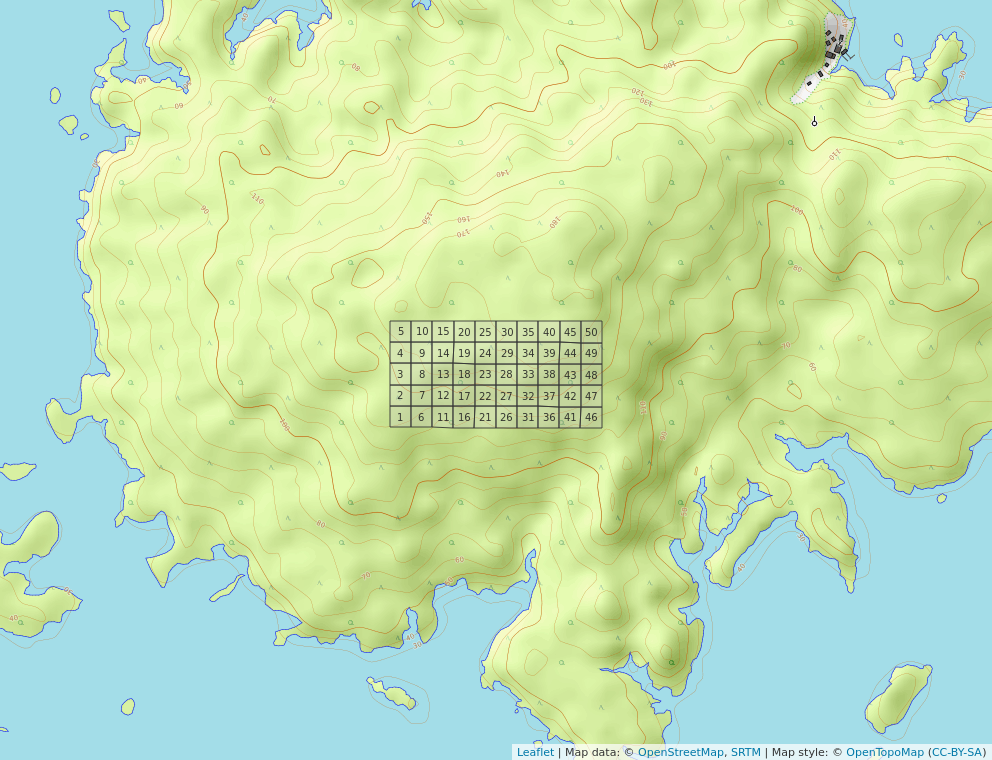
\includegraphics{mapa_cuadros.png}
\caption{\label{fig:mapa_cuadros}Organizacion de la parcela por
cuadricula de una hectarea}
\end{figure}

\ldots

\section{Resultados}\label{resultados}

El censo de 2010 de la parcela permanente de la Isla Barro Colorado
indica que la familia Euphorbiaceae consta con 10 especies y un total de
2421 individuos. La más rara, es decir, la menos abundante, fue
\emph{Alchornea latifolia}, con un solo individuo, seguida de
\emph{Sapium broadleaf} con dos individuos. La más abundante fue
\emph{Acalypha diversifolia}, con 1023 individuos (ver tabla
\ref{tab:tabla_de_abundancia} y figura \ref{fig:abun_sp_q}). La
distribución de la riqueza y la abundancia por sitios es desigual, con 6
especies y ca. 50 individuos en promedio por cuadros de 1 Ha. Los
valores mínimo y máximo de riqueza y abundancia por sitios muestran que
se trata de una familia con mucha variabilidad en la parcela; en los
cuadros 10, 17 y 43 se registraron tan sólo tres especies, mientras que
en los cuadros 29 y 37 se registraron 8. Asimismo, la abundancia por
cuadros fue muy variable, registrándose en el cuadro 2 el valor de
abundancia mínima de 7 de individuos y un máximo de 162 individuos en el
cuadro 50.

\begin{longtable}[]{@{}lr@{}}
\caption{\label{tab:tabla_de_abundancia}Abundancia por especie de la
familia Euphorbiaceae}\tabularnewline
\toprule
Latin & n\tabularnewline
\midrule
\endfirsthead
\toprule
Latin & n\tabularnewline
\midrule
\endhead
Acalypha diversifolia & 1023\tabularnewline
Croton billbergianus & 631\tabularnewline
Alchornea costaricensis & 316\tabularnewline
Adelia triloba & 143\tabularnewline
Hieronyma alchorneoides & 118\tabularnewline
Hura crepitans & 95\tabularnewline
Acalypha macrostachya & 52\tabularnewline
Sapium glandulosum & 40\tabularnewline
Sapium broadleaf & 2\tabularnewline
Alchornea latifolia & 1\tabularnewline
\bottomrule
\end{longtable}

Analizando la siguiente gráfica que nos indica la distribución y
presencia de cada especie de Euphorbiaceae presente en esta zona de
trabajo,en donde a mano izquierda están las especies encontradas y de
forma longitudinal las 50 hectáreas.Lo que vemos es que \emph{Acalypha
diversifolia} , es la especie más abundante ya que registró un muchos
individuos por cuadros de esta especie seguido de \emph{Croton
billbergianus}. Un dato más que nos arroja esta tabla es que estas
mismas especies pueden coexistir ya que se les ve en algunas cuadrículas
en las que ambas coinciden con una alta cantidad de individuos, estas
cuadrículas corresponden a la 23 y a la 50, mismas que poseen la mayor
riqueza global de la parcela (ver
figura\ref{fig:cuadro_riqueza_global}Riqueza global)Todo esto nos guia
no solo a ver la riqueza por individuo si no que tambien por familia.

\begin{figure}
\centering
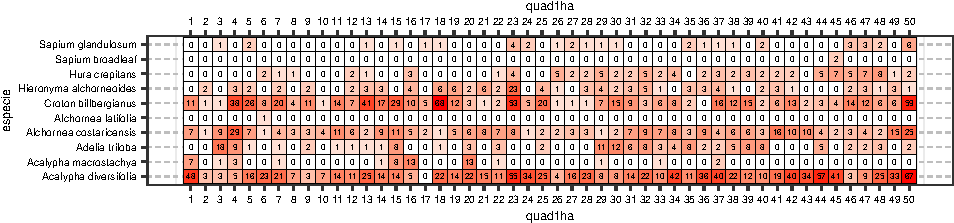
\includegraphics{manuscrito_files/figure-latex/unnamed-chunk-3-1.pdf}
\caption{\label{fig:abun_sp_q}Abundancia por especie por quadrat (a la
izquierda esta la lista de especies y a mayor intenso el color de la
cuadricula, mayor es el numero de individuos}
\end{figure}

Continuando con la abundancia, esta vez veámoslo desde la perspectiva de
familias, el mapa que nos orienta nos da una ventaja y es que nos brinda
la perspectiva de de las variaciones del relieve de la parcela. Lo
primero en resaltar es que las cuadrículas 23 y 50, las mismas que tiene
el mayor número de especies(\emph{cómo referenciar esa tabla}) y las que
poseen mayor riqueza global, (ver figura\ref{fig:cuadro_riqueza_global})
resaltan una vez más, no son las que más poseen pero son de las que más
poseen familias por cuadrículas con 6 y 7 familias de forma consecutiva.
La mayor abundancia de familias está presente en las cuadrículas 29 y 37
con 8 familias por cuadrículas, cabe destacar que aunque no sean
continuas con relación a su posición, ambas entran en la categoría de
bosque viejo en relieve alto (más adelante veremos esta y otras
categorías con más detalle). Esto abre una puerta a más variables
determinantes que influyen el la presencia, distribución y riqueza de
las especies,esto se debe a que la variación del relieve, tipo de
vegetación, influye directamente el clima, humedad, suelo, temperatura y
muchos más factores que son imprescindibles para la presencia de ciertas
especies, esto aplica para todo ser vivo, no de forma exclusiva a
Euphorbiaceae.

(ver figura \ref{fig:cuadro_de_riqueza_familia})

\begin{figure}
\centering
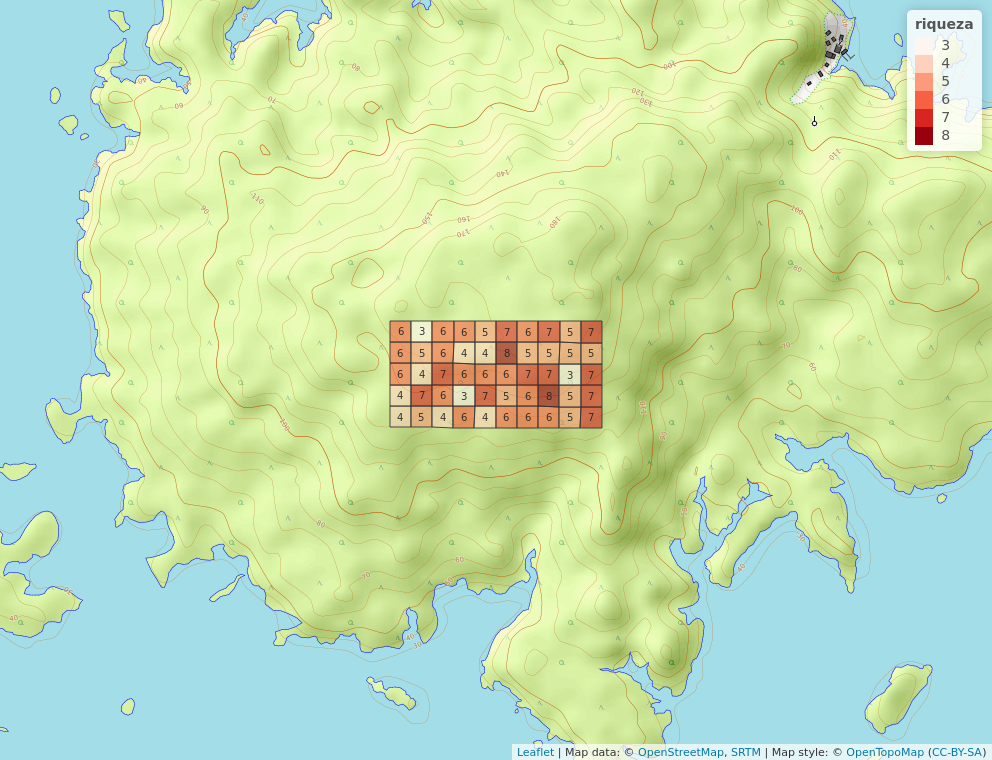
\includegraphics[width=0.50000\textwidth]{mapa_cuadros_riq_mi_familia.png}
\caption{\label{fig:cuadro_de_riqueza_familia}Representacion de la
riqueza de la familia Euphorbiaceae por cuadricula de una hectarea}
\end{figure}

La riqueza global de la flora de barro colorado muestra una asosiacion
entre la abundancia y las pendientes y zonas altas, mas que en las zonas
de transicion, segun el mapa de abundancia global.En las inclinaciones
noroeste y una parte del este,se encuentran las cuadriculas con mayor
cantidad de individuosy oxcialan desde los 4,500 a los 51014.Aun asi las
demas cuadriclas muestran bastante presencia de individuos, todas las
cuadriculas sobrepasan los 2,000, especificamente en las zonas centricas
de la parcela. A un asi, mas que determinar un patron, la aubundancia es
bastante homogenea respecto a cada cudricula (puntos cardinales)

(ver figura\ref{fig:cuadro_riqueza_global})

\begin{figure}
\centering
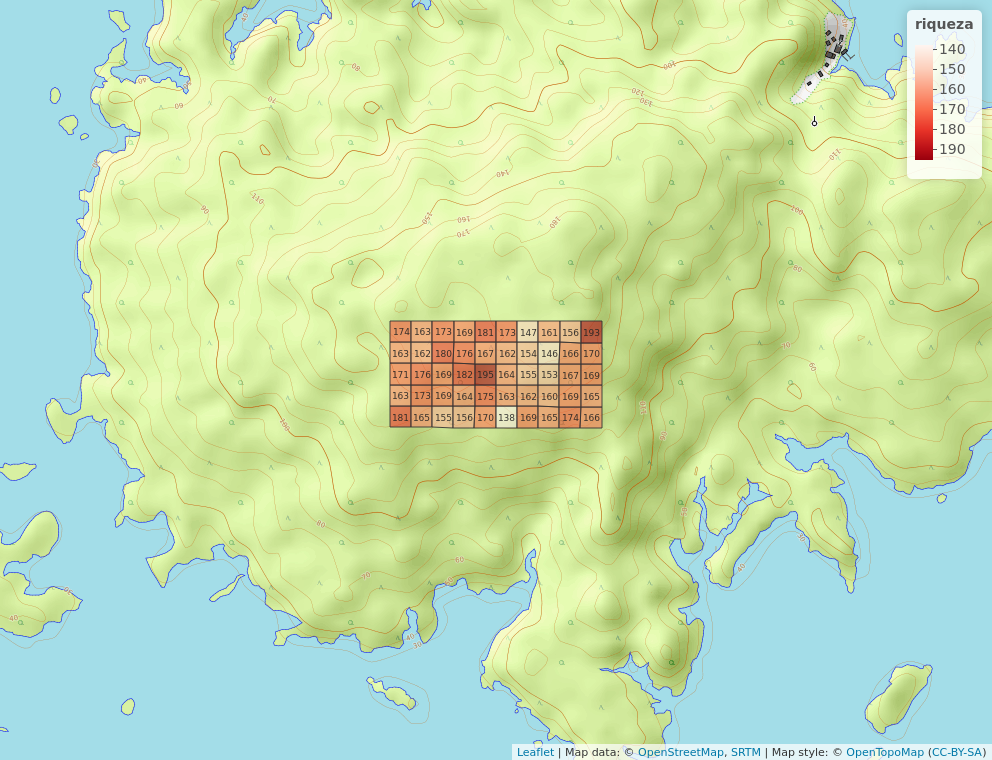
\includegraphics[width=0.50000\textwidth]{mapa_cuadros_riq_global.png}
\caption{\label{fig:cuadro_riqueza_global}Riqueza global}
\end{figure}

Comparando la abundancia global de nuestra familia de trabajo con la
abundancia global de especies podemos notar lo siguiente, existe una
asociación entre la abundancia global de especies y la abundancia global
de Euphorbiaceae y la inclinación, ya que las cuadrículas con mayor
cantidad de individuos también están situadas en la parte noroeste de la
parcela y la parte este también.

(ver figura \ref{fig:cuadro_de_abundancia_global})

\begin{figure}
\centering
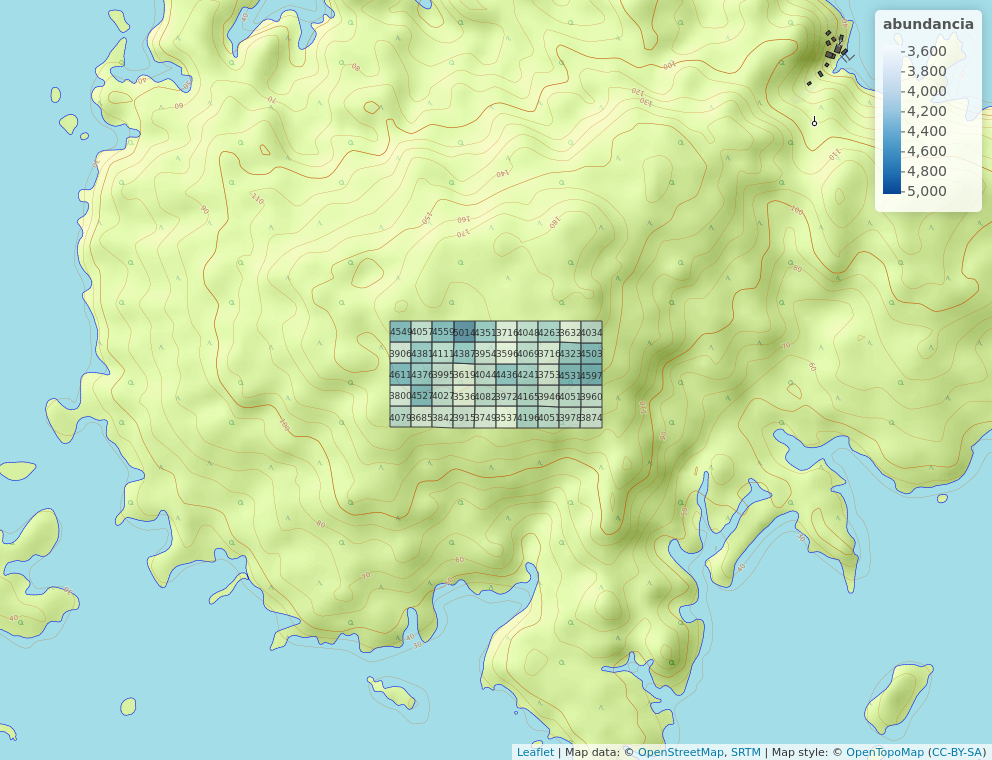
\includegraphics[width=0.90000\textwidth]{mapa_cuadros_abun_global.png}
\caption{\label{fig:cuadro_de_abundancia_global}Abundancia global}
\end{figure}

En cuanto a la abundancia de Euphorbiaceae, la a cuadrícula 50 es la que
posee mayor cantidad de individuos seguido de la número 23 que se ubica
en la parte céntrica de la parcela con 147 individuos. En el mapa de
abundancia global se muestra el mismo patrón(ver figura
\ref{fig:cuadro_de_abundancia_global}), donde la cuadrícula 28 también
situada de forma céntrica, es una de las cuadrículas con más individuos,
4,436 para ser exactos, lo que me permite llegar a la conclusión que la
abundancia global de Euphorbiaceae está asociada a la inclinación del
relieve y la abundancia global de especies. Puede que haya un tercer
factor ( altitud, nutrientes, tipo de suelo,microclima,etc) que
determine la alta presencia de especies en esta zona y a la vez la alta
presencia de Euphorbiaceae.

(ver figura\ref{fig:cuadro_abundancia_de_mi_familia})

\begin{figure}
\centering
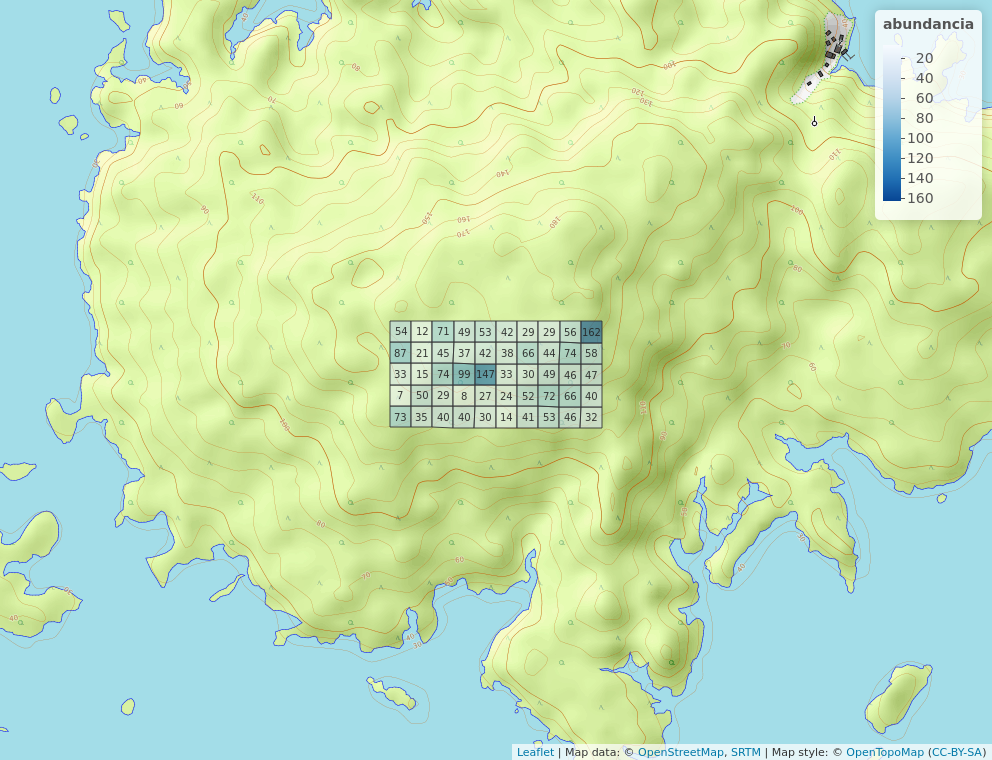
\includegraphics[width=0.85000\textwidth]{mapa_cuadros_abun_mi_familia.png}
\caption{\label{fig:cuadro_abundancia_de_mi_familia}Abundancia de
Euphorbiaceae}
\end{figure}

En el análisis de correlación de la riqueza y la abundancia de
Euphorbiaceae, sólo se detectó un patrón destacable: el contenido de
hierro del suelo presenta relación positiva y significativa con la
abundancia, no así con la riqueza. Son igualmente destacables, las
significativas asociaciones negativas y positivas que existen entre
distintas variables de suelo, aunque es común que múltiples variables de
suelo interactúen entre sí (ver figura \ref{fig:suelo_ph_abun_riqu})

\begin{figure}
\centering
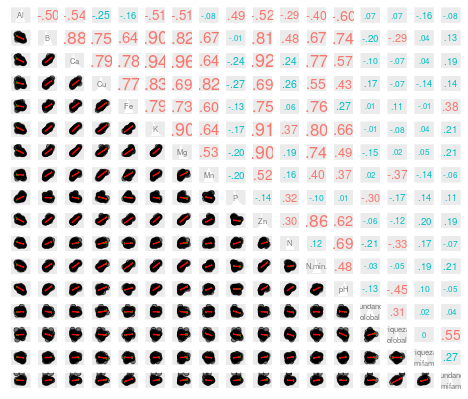
\includegraphics{suelo_ph_abun_riqu.png}
\caption{\label{fig:suelo_ph_abun_riqu}Relacion de elementos y ph del
suelo con la riqueza y abundancia de especies}
\end{figure}

Viendo la riqueza y abundancia desde una perspectiva de heterogenidad
ambiental, segun Pearson tomando en cuenta la geomorfologia y los que
observamos es que hay avriables como la elevacion o la pendiente media
que muestran asociacion con muchas de las variables del analisi, pero
los aspectos que nos interesan son relacion entre la abundancia y
riqueza de Euphorbiacea con las demas variables del analisis, y como
resultados tenemos que la abundancia de Euphorbiaceae muestra asociacion
con la riqueza gobal de especies, al igual que con la pendiente media,
geomorfologia de valle y la heterogenidad ambiental, mientras que la
riqueza de nuestra familia solo muestra relacion con con la
heterogenidad ambiental y a diferencia de la abundancia no muestra
relacion alguna con la riqueza global.\\
(Ver figura\ref{fig:geo_pearson})

\begin{figure}
\centering
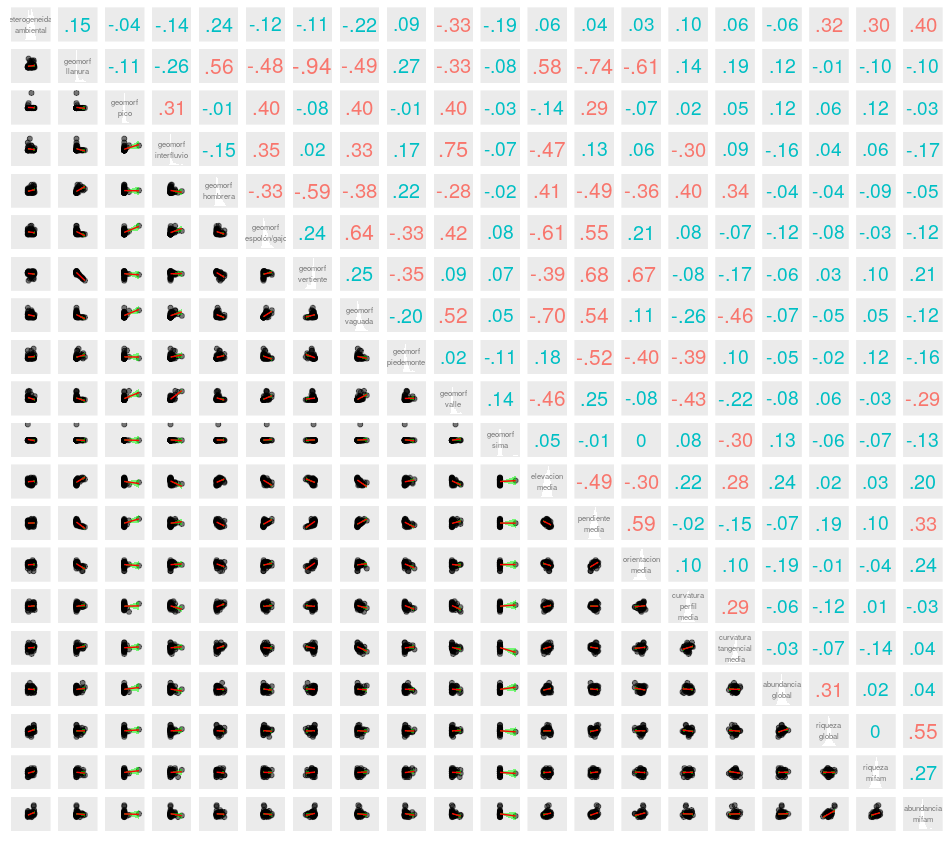
\includegraphics{geo_pearson.png}
\caption{\label{fig:geo_pearson} Relacion entre la Heterogenidad y
geomorfologia con respecto a la abundancia y riqueza de Euphorbiaceae
según Pearson}
\end{figure}

Pero desde la perspectiva de Spearman

(ver figura\ref{spearman})

\begin{figure}
\centering
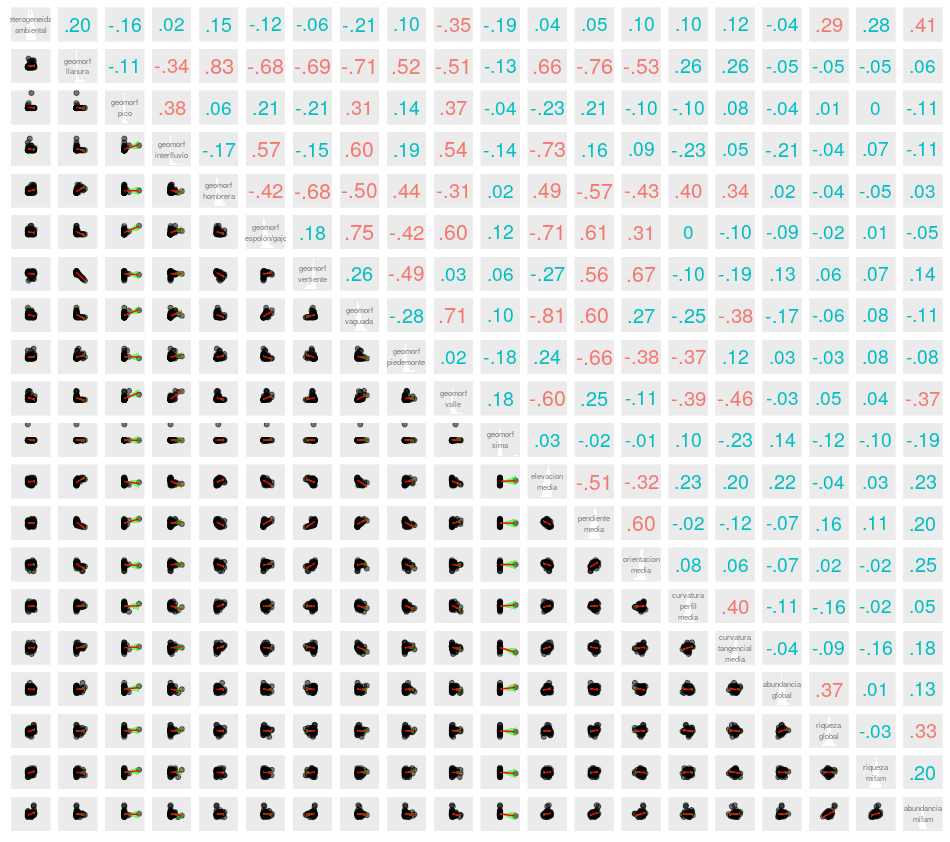
\includegraphics{spearman.png}
\caption{\label{fig:spearman}Relacion entre la Heterogenidad y
geomorfologia con respecto a la abundancia y riqueza de Euphorbiaceae
según Spearman}
\end{figure}

MEDICIÓN ASOCIACIÓN

Lo que vemos a continuación es la interpretación visual de la matriz de
distancia euclídea calculada a partir de la matriz de comunidad
transformada por el método de Hellinger, revela que existen al menos
tres clusters claramente diferenciados (ver
figura\ref{fig:matriz_disimilaridad_hellinger}). Un clúster grande
integrado por al menos 17 sitios (e.g.~sitios 25, 32, 33, 37, 50). Un
segundo cluster más pequeño de unos 4 sitios \emph{el 41 va}
(e.g.~10,8,42,49) y un terce cluster compuesto por las cuadriculas
\emph{36?},28,27,45,6,48,44,34 y 39. (lea la representación de cada
color al pie de la gráfica para una mayor interpretación) Para llegar a
esta conclusión, se tomó en cuenta la distancia entre los sitios, dígase
la disimilaridad (a mayor distancia, mayor disimilaridad), la cual se
representa usando la métrica de la distancia euclídea(explica qué es),
lo que equivale a una matriz de comunidad transformada, en este caso a
una matriz de Hellinger, ésta se representará de forma gráfica en un
mapa de calor con diversos colores, el 1er mapa no representa ningún
orden, mientras que el 2do sí, facilitando así determinar patrones o
grados de asociación.

(ver figura\ref{fig:diss_hellinger})

\begin{figure}
\centering
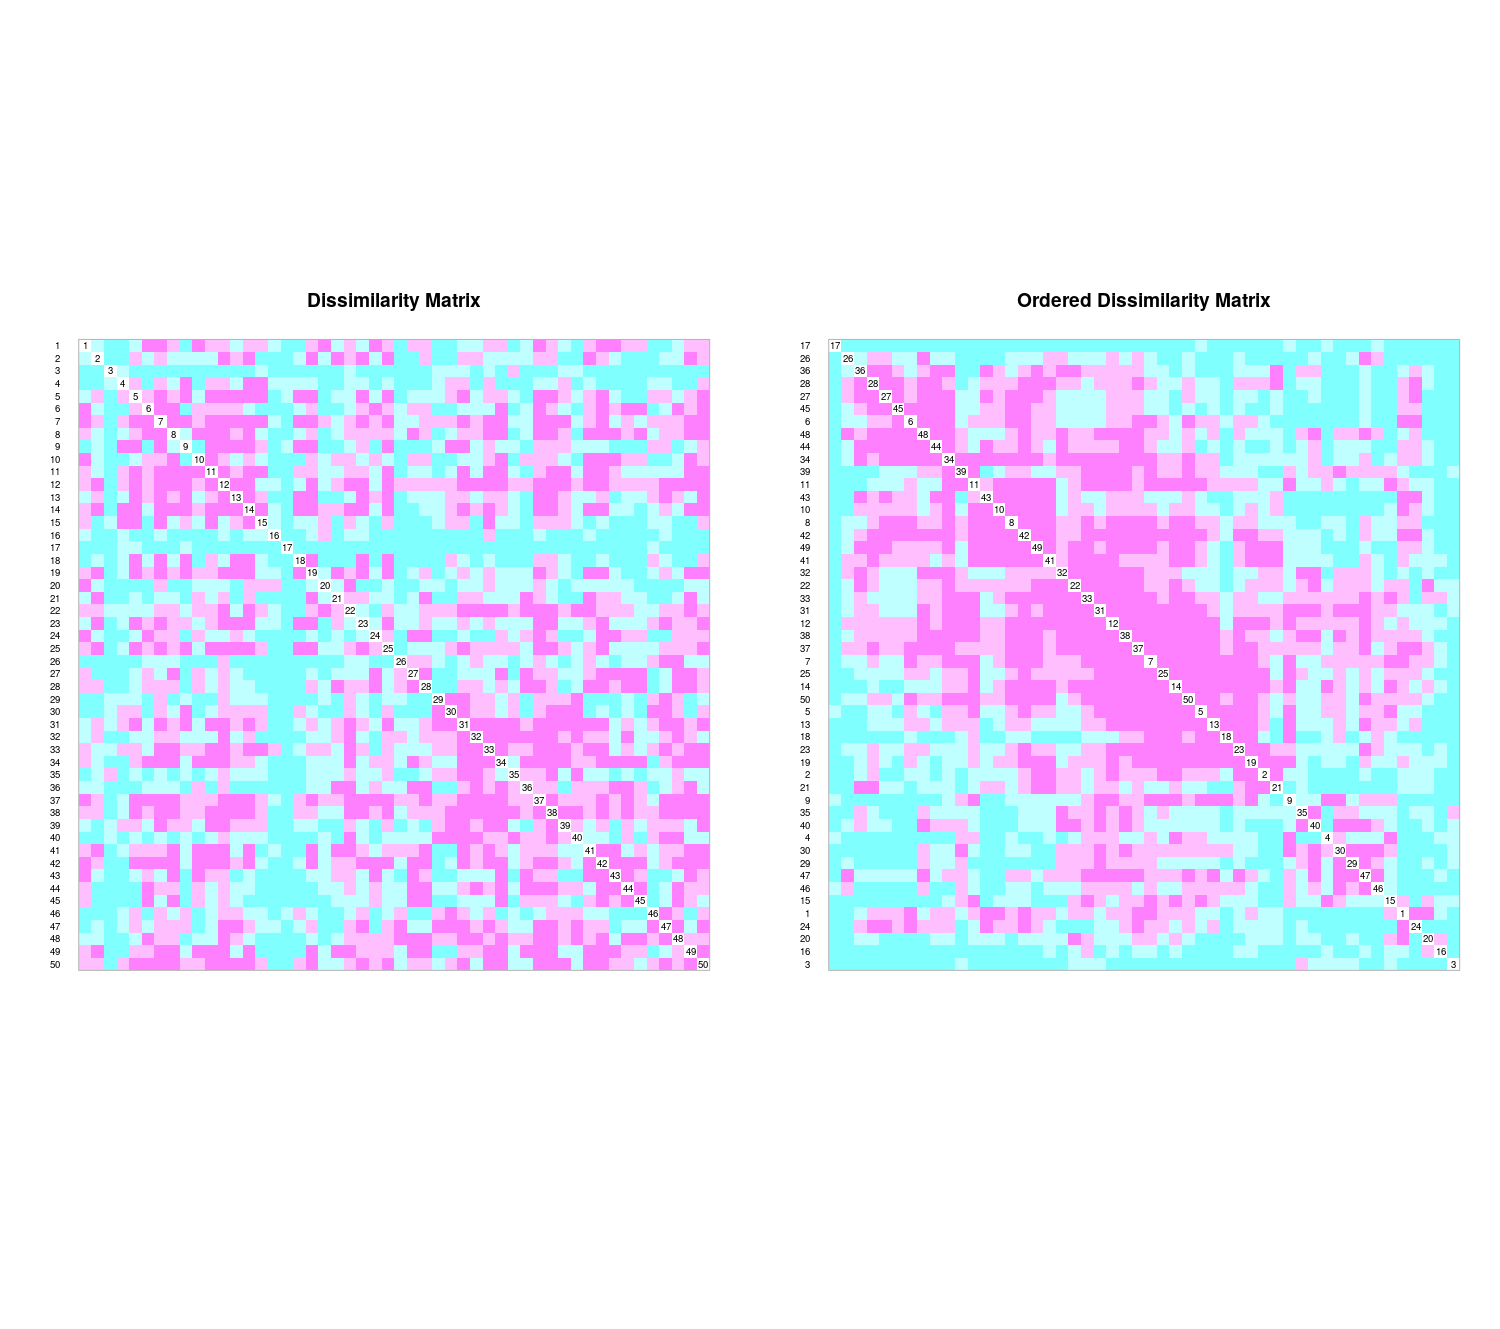
\includegraphics{diss_hellinger.png}
\caption{\label{fig:diss_hellinger}Matriz de Disimilaridad de
Hellinger,Rosa intenso:muy cerca, lila o rosa claro: distancia
intermedia;estan cerca, azul celeste o turquesa:larga distancia,
blanco:cero, un punto comparado consigo mismo}
\end{figure}

Los puntos x y x guardan asociación compartida en cuanto a sus especies
compartidas, lo que significa que desde el punto de vista de Jaccard
estos puntos están muy próximos.Lo mismo pasa con los puntos x x x xy x

En conclusión, la zona de trabajo muestra un 91.7\% de similaridad o
especies compartidas.

(Ver figura\ref{fig:diss_jaccard})

\begin{figure}
\centering
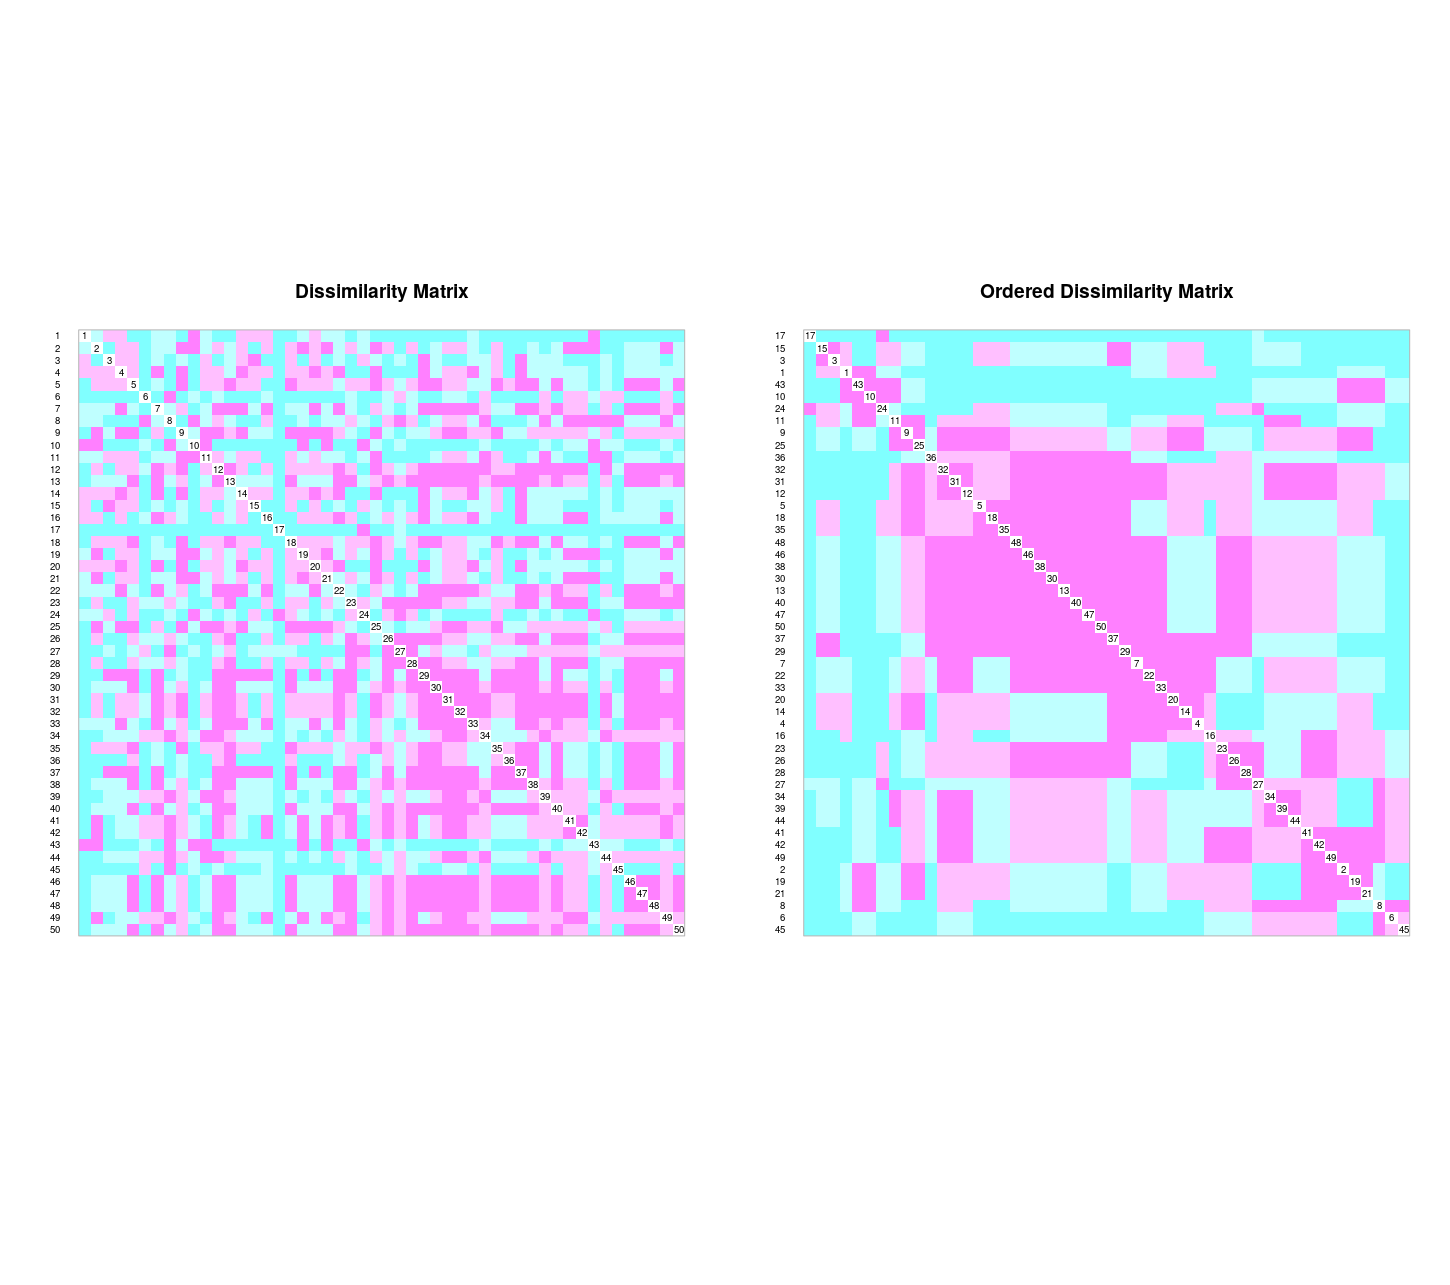
\includegraphics{diss_jaccard.png}
\caption{\label{fig:diss_jaccard}Matriz de disimilaridad de jaccard}
\end{figure}

Estas es mas una matriz mixta ya que tomaremos en cuenta tanto variables
cuantitativas como las cualitativas para nuestro análisis de distancia a
partir de la heterogeneidad ambiental, dígase qué tan homogéneos son los
micro hábitat en las cuadrículas o hectáreas, el tipo de hábitat y
quebrada,presencia o ausencia de cañada (tabla de 3 columnas en nuestro
script de análisi) Con relación a la topografía usaremos Old High
(bosque viejo en relieve alto), Old Low(bosque en vertiente baja), Old
Slope(bosque relieve bajo), Swamp(bosque en área encharcable) y
Young(bosque joven). Los resultados interpretados en base a la columna
en el script y la matriz son: Los niveles de heterogeneidad con respecto
a microhábitat son bajos y pueden ir desde 0.0000 a 0.6368, lo que nos
dice que existe una gran homogeneidad entre las microhábitat las
hectáreas. Con relación al hábitat, los más escasos son Swamp o bosque
en área encharcable y Young o bosque joven, en 1ro solo se encuentra en
las cuadrículas 23 y 18 lo que resulta razonable ya que ambas posiciones
están contiguas de forma longitudinal en la parcela, mientras que young
o bosque joven está en las cuadrículas 30 y 35 que al igual que la
anterior, están de formas continuas de forma longitudinal(el 23 a la
derecha del 15), puedes visitar la referencia 1 donde muestra la
organización de la parcela por hectárea y ubicar estos puntos para
entender mejor. (Ver figura\ref{fig:mapa_cuadros}Organización de la
parcela por cuadrícula de una hectárea) Las cuadrículas que coinciden
con Old Slope son :cuadrícula 1,5,16,21,26,36,41,42,43,44,45,46 y 50.
Las cuadrículas 1 y 5 están en extremos opuestos, la 16 y 21 están
contiguas de forma horizontal, lo mismo pasa con la 26 y 36 aunque estas
tienen la cuadrícula 31 de por medio que posee un tipo de bosque
diferente a estas, Ludlow para ser específicos, las 41,42,43,44,45
forman una una línea vertical con respecto a la hectárea teniendo a las
cuadrículas 46 y 50 en cada extremo de esta línea, también resaltar que
en las cuadrículas 1 y 50 hay presencia de quebrada. Tipo de bosque Old
High está presente en las cuadrículas 29,32,33,34,37,38,39 y 40, desde
la 32 a la 34 están posicionadas de forma vertical, esta última con la
29 a su derecha y desde la 37 a la 40 también formas una línea vertical
con respecto a la parcela. EL tipo de bosque más abundante fue Hollow,
tipo de bosque en vertiente bajo quebrada\ldots{}.

Debemos recordar que tanto abundancia como la riqueza de nuestra familia
esta asociada a la heterogenidad ambiental segun la correlacion de
Pearson.

hay cambios bruscos de tipo de bosque a pesar de la homogeneidad de la
parcela??

(Ver figura\ref{fig:punt_z})

\begin{figure}
\centering
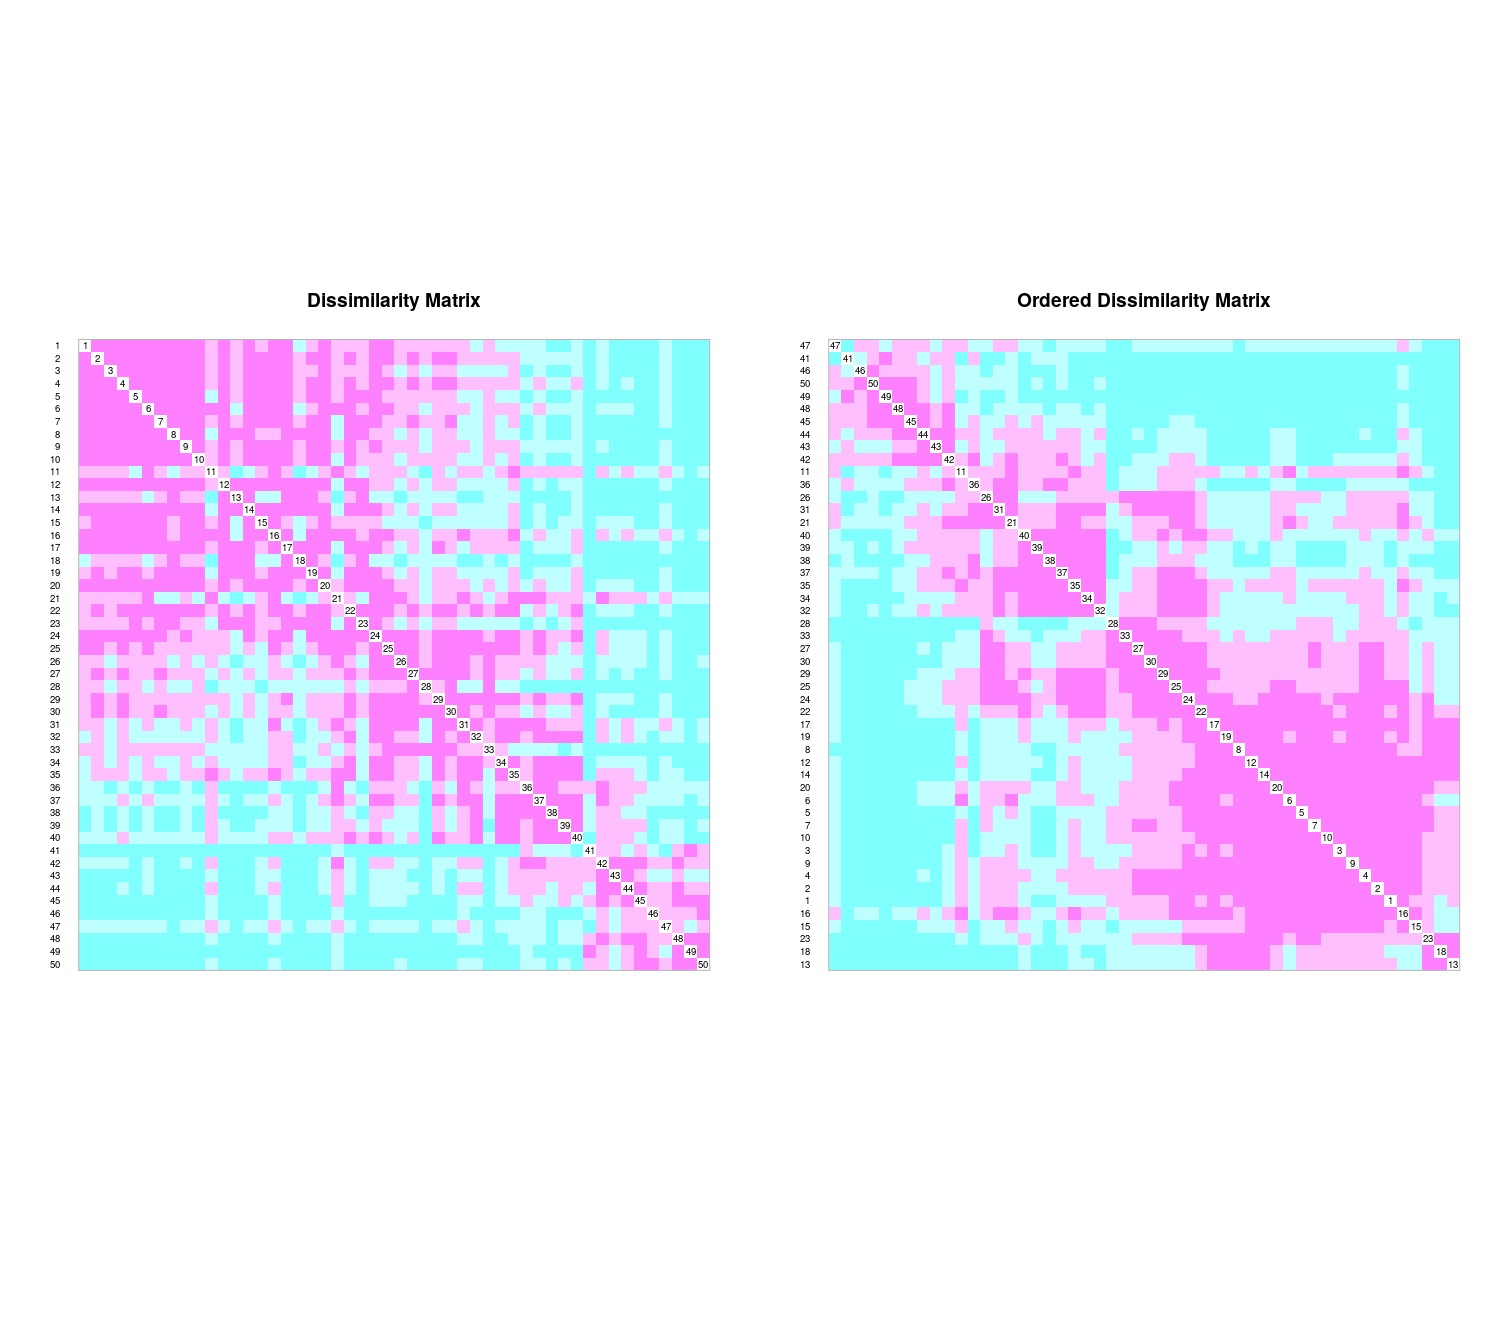
\includegraphics{punt_z.png}
\caption{\label{fig:punt_z}Matriz mixta}
\end{figure}

Una vez analizada la heterogeneidad, veamos el grado de asociación entre
especie no sitio, o dicho de otra manera, presencia ausencia de especies
a través de un cálculo de la distancia euclídea.

Esto se hace a través de una matriz transpuesta usando datos de
abundancia, para ver la posible asociación o patrones las medidas o
distancia de las especies. Cabe destacar que estos datos también se
analizaron mediante la \emph{Correlacion de Pirson}, usando una matriz
de comunidad en modo R, donde dicha matriz se convirtió en datos
binarios y los resultados ``brutos'' que arrojó mostraron consistencia,
pero vemos los resultados de esta y comparemos.

(Ver figura\ref{fig:asoc_esp_no_sitio})

\begin{figure}
\centering
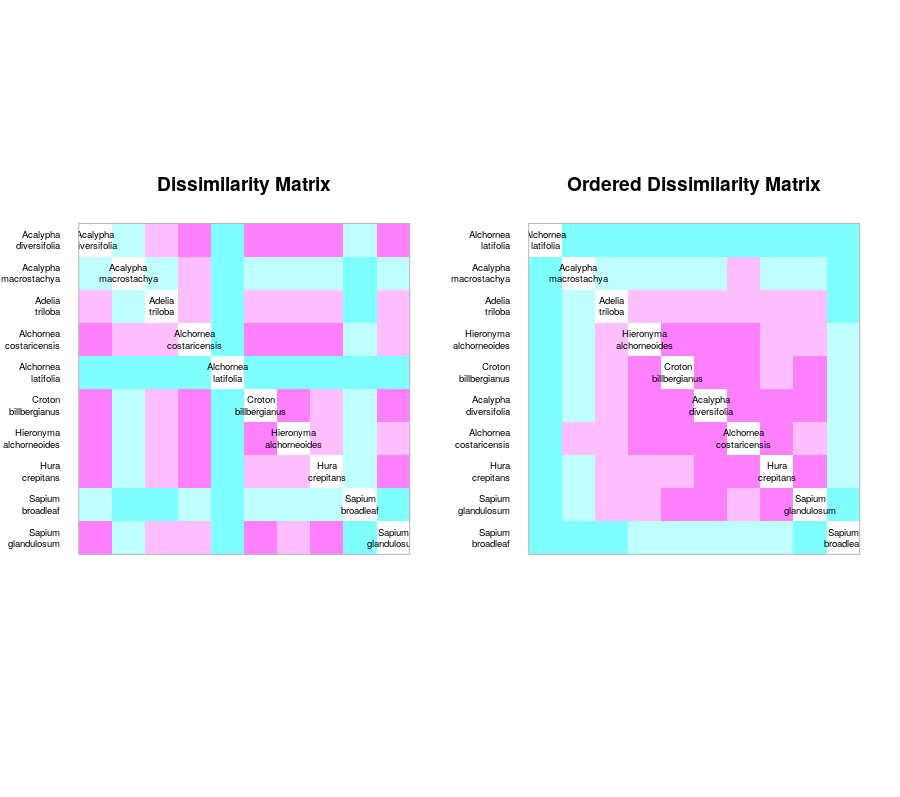
\includegraphics{asoc_esp_no_sitio.png}
\caption{\label{fig:asoc_esp_sitio}Presencia ausencia}
\end{figure}

Lo primero que podemos resaltar es que esta matriz nos muestra que
\emph{Alchornea latifolia} no muestra asociación o cercanía con las
demás especies, siendo así de las que más distancia muestra con relación
a las especies,mientras que \emph{Alcalypha macrostachya} es la que
menor distancia guarda entre especies no sitio. También nos muestra un
cluster de especies que se correlacionan, guardando una gran cercanía
entre sí, tales como \emph{Hieronyma alchorneoides} con \emph{Croton
billbergianus}, esta última con \emph{Acalypha diversifolia} etc. Aunque
esto es de gran utilidad, una perspectiva que también nos es de gran
utilidad es la correlación pero basada en nutrientes y elementos del
suelo.

TECNICA DE ORDENACION NO RESTRINGIDA

Es importante ver si el ph y otros elementos del suelo se correlaciona
con nuestras especies, y esto podemos hacerlo a través de análisis de
PCA o análisis de componentes principales, CA o análisis de
correspondencia y PCoA o análisis de coordenadas principales, cada una
sus siglas en inglés.Estos nos servirán para ver el grado de asociación
que guardan los sitio y elementos del suelo. Debemos recordar que la
ordenación se basa también en la similaridad y que su principal
propósito es procurar reducir la dimensionalidad de los datos a través
de un conjunto de técnicas, como representar datos en ejes ortogonales
(comúnmente dos),donde el eje 1 explica la mayor varianza, el eje n
explica la mínima, etc.

Comencemos por PCA en un modelo de vara quebrada, pero antes aclarar que
la ordenación en este caso también se basa en la similaridad y que su
principal propósito es procurar reducir la dimensionalidad de los datos
a través de un conjunto de técnicas, como representar datos en ejes
ortogonales (comúnmente dos),donde el eje 1 explica la mayor varianza(la
mayor cantidad de varianza posible en el menor número de ejes), el eje n
explica la mínima, etc en este todas nuestras variables son numéricas y
comparables en cuanto a la escala de medición se refiere. los resultados
obtenidos a través de este análisis de componentes principales son los
siguientes:

(ver figura\ref{fig:PCA_1})

\begin{figure}
\centering
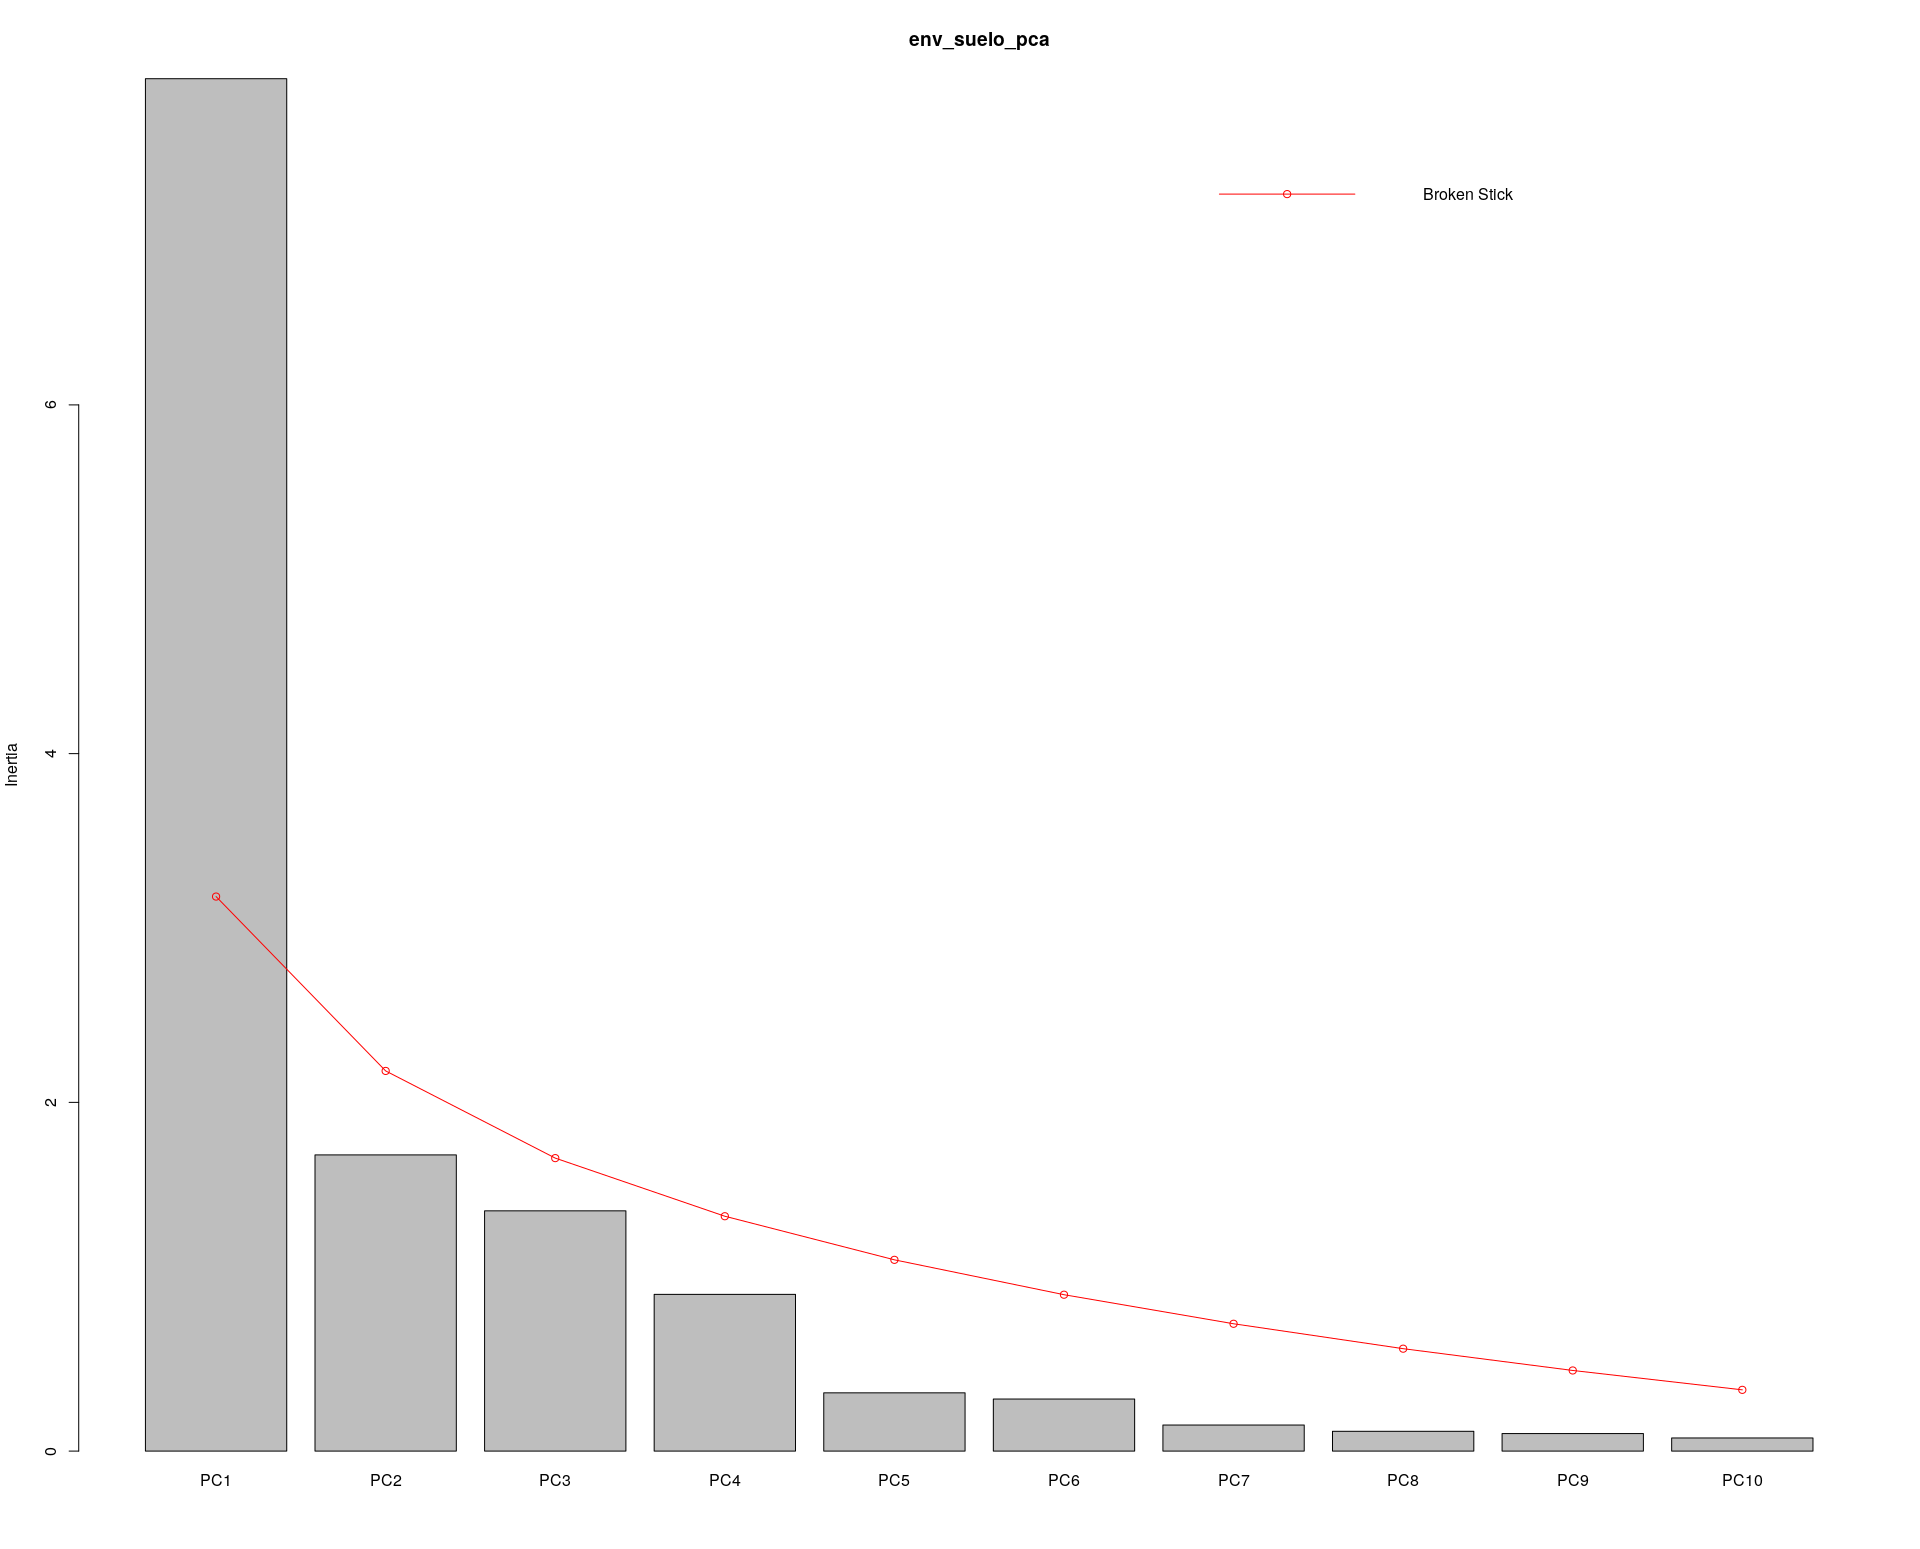
\includegraphics{PCA_1.png}
\caption{\label{fig:PCA_1}Presencia ausencia(Las barras representan los
valores propios de nuestros datos en cada una de las componentes y la
liena roja la vara quebrada)}
\end{figure}

Nuestro análisis de componente principal aplicado a la matriz de suelo
nos dice que el componente PC1 es importante y el resultado que nos
arroja es más de lo que se podría esperar para un modelo de vara
quebrada, un poco más que el doble, y que aporta suficiente varianza
para nuestra matriz, a diferencia de los demás componentes que no
sobrepasan la vara quebrada lo que nos indica que esos componentes son
pocos útiles ya que no consiguen explicar lo suficiente.

Viéndolo desde otra perspectiva, digase desde un Biplot, la correlación
se vería de esta forma: Podemos interpretar los datos de la siguiente
manera: la distancia euclídea está preservada en el escalamiento 1 y pH,
P y N son los componentes de suelo más abundantes en este escalamiento,
estos contribuyen mucho más en los componentes 1 y 2 y que en el resto
de los componentes,dígase poco equitativo, mientras que los demás
elementos o descriptores tiene una contribución para los demás los
componentes más o menos homogénea para cada uno de los sitios . En el
escalamiento 2(distancia de majala novis), el pH y el Nitrógeno guardan
una relación con los sitios 31,35,3637,38,39,40, mientras que ,
minerales como el hierro (Fe) y el aluminio (Al), están presente en casi
el 50\% de los sitios, siendos así muy parecidos en términos de
suelo(negativo). Otros puntos a resaltar son que los elementos Cu, Mn,
Fe están muy asociados, al igual que K y Zn, Ca,Mg Y N.min. lo que
significa que cuando uno crece el otro también, a diferencia de B y Al o
de P y Fe que cuando uno crece el otro disminuye porque no guardan
relación entre sí en otras palabras una relación inversa.

Agrupamiento basados en la distancia euclídea con los datos escalados

(ver figura\ref{fig:Biplot_pca1_pca2})

\begin{figure}
\centering
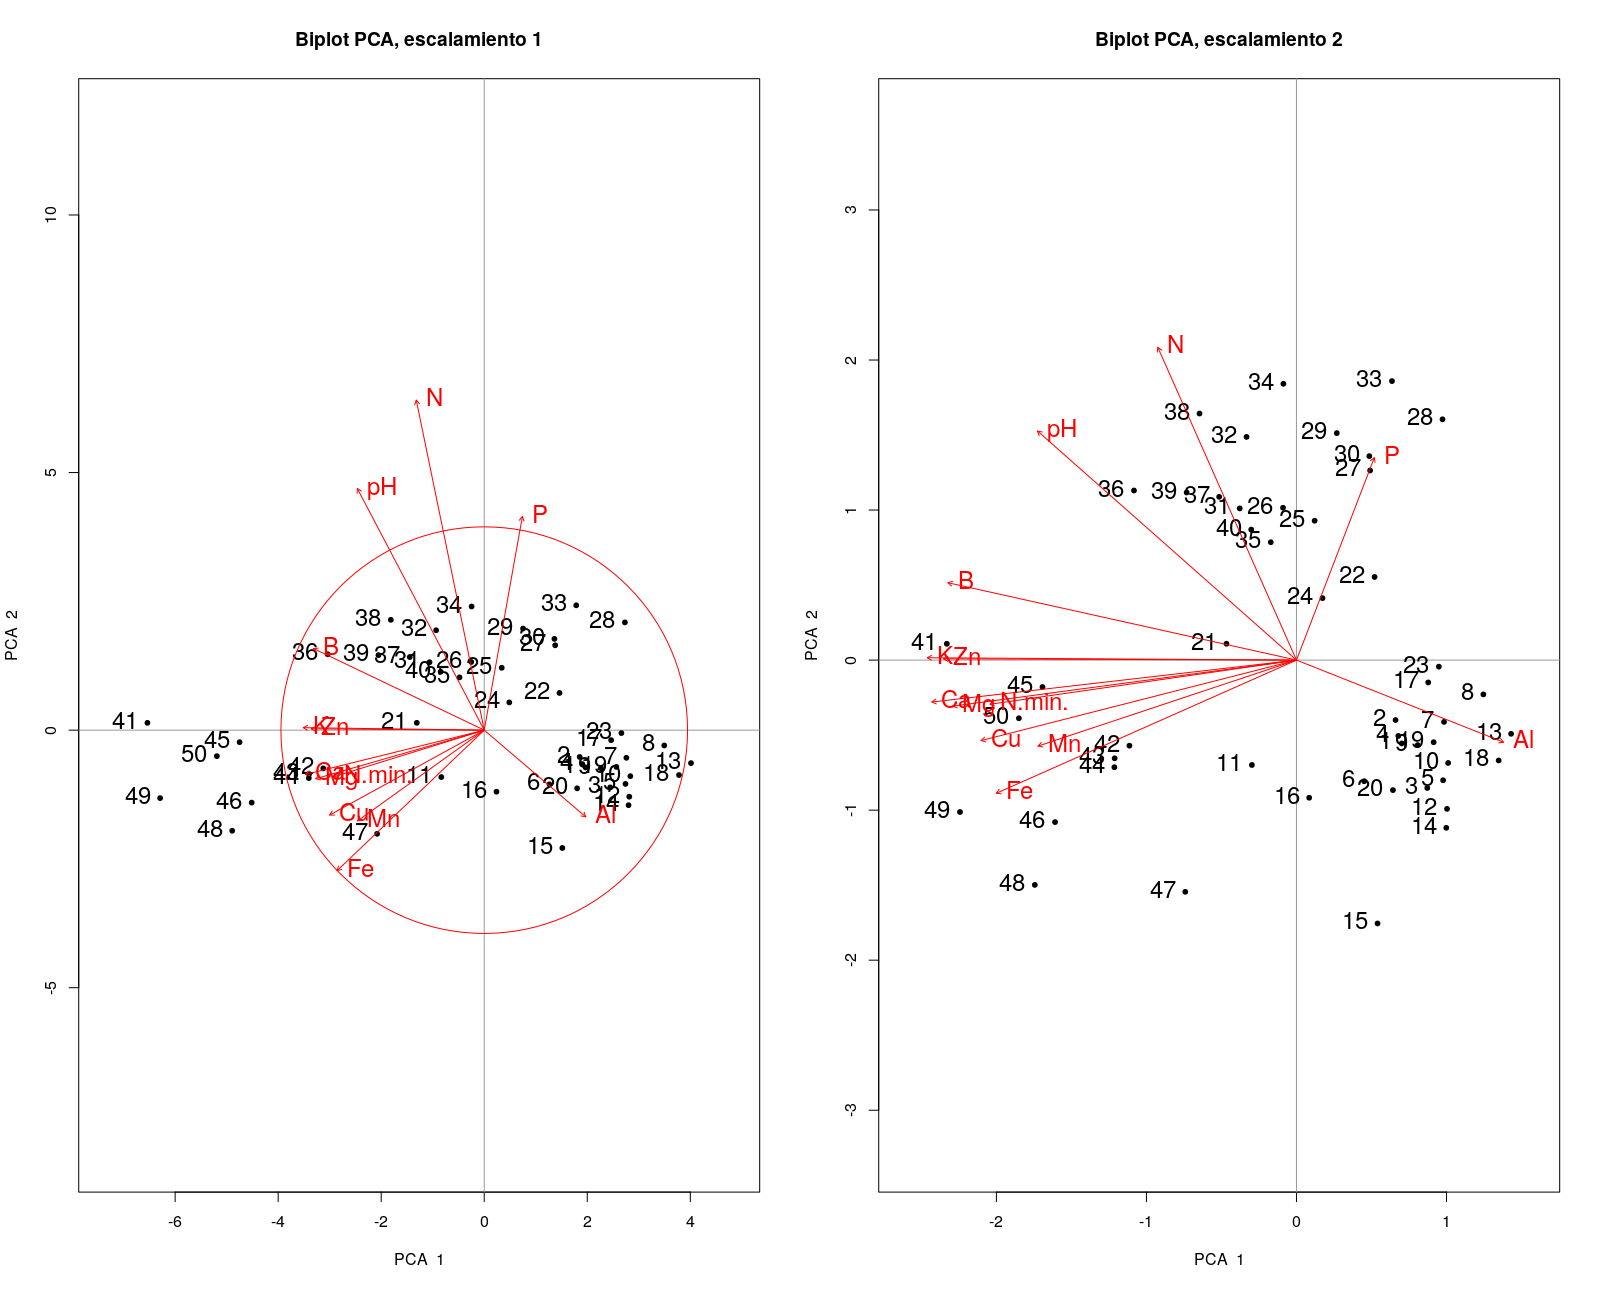
\includegraphics{Biplot_pca1_pca2.png}
\caption{\label{fig:Biplot_pca1_pca2}Recordae que el angulo entre los
vectores el lo que indica la correlacion estre ellos y que los sitiios
estan representados por puntos}
\end{figure}

Aunque las escalas son diferentes, podríamos decir que el patrón se
mantiene en ambos escalamientos ya que se presenta un agrupamiento de 3
cluster en ambos Biplot. aquí puedes ver un el conjunto de cluster en
función de los mismos datos de suelo, esta consistencia resulta
razonable aunque los métodos de ordenación no sean los mismos ya que
ambos se basan en la distancia euclídea.

(ver figura\ref{fig:cluster_pca})

\begin{figure}
\centering
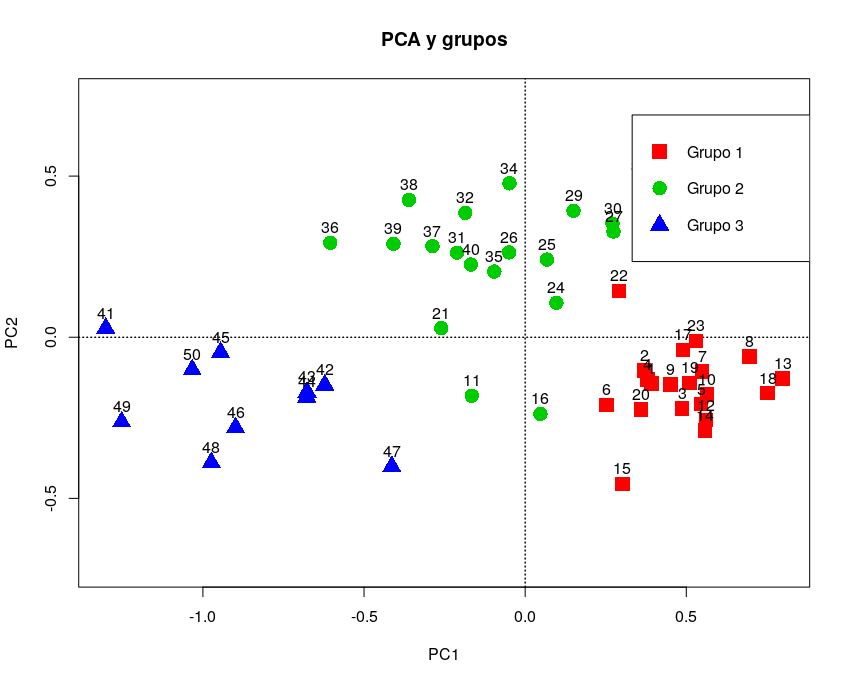
\includegraphics{cluster_pca.png}
\caption{\label{fig:cluster_pca}leyenda aqui}
\end{figure}

Si aplicaramos en análisis de PCA para especies y no para variables
obtendremos ;lo siguiente: Nuestro modelo de vara quebrada quedaría de
la siguiente manera: el componente 1 a diferencia que el de datos de
suelo,este tiene poco más de lo que se podría esperar para el modelo de
vara quebrada, lo mismo pasa con el 2do componente pero en los demás no,
siendo estos dos primeros imprescindibles para el análisis de la matriz
de comunidad.Aun asi se podrian usar las primeras 4 o 5 componentes para
una mayor comprensión.

(ver figura\ref{fig:quebrada_especie})

\begin{figure}
\centering
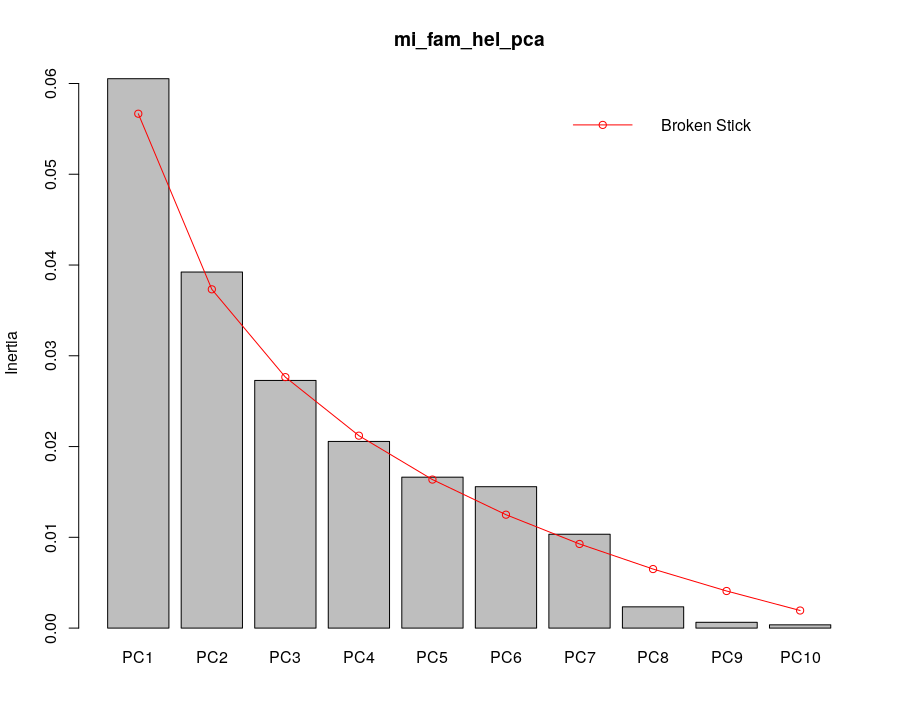
\includegraphics{quebrada_especie.png}
\caption{\label{fig:quebrada_especie}leyenda aqui}
\end{figure}

Viéndolo desde la perspectiva de diagrama de escalamiento o biplot,
obtendremos lo siguiente: (ver figura\ref{fig:biplot_especie})

\begin{figure}
\centering
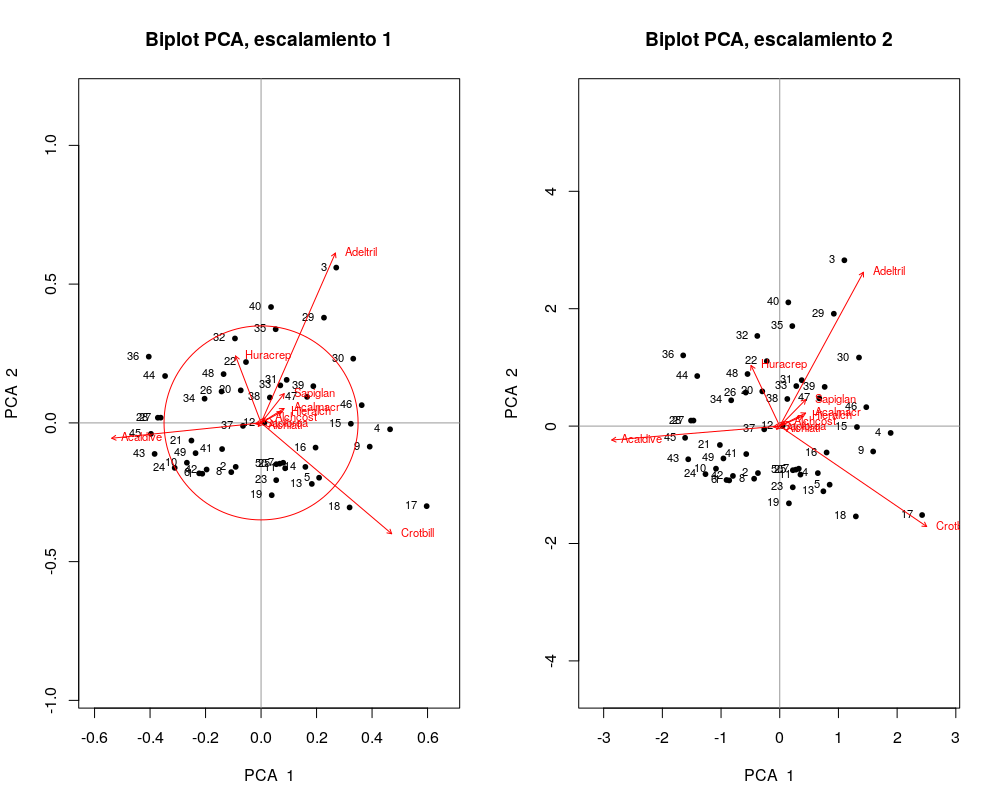
\includegraphics{biplot_especie.png}
\caption{\label{fig:biplot_especie}leyenda aqui}
\end{figure}

Es de esperarse que los patrones no coincidan con el diagrama de
escalamiento anterior o biplot, y esto es porque las variables que se
están tomando en cuenta son diferentes. Anteriormente se usaban
elementos de suelo como descriptores y en este caso las especies de
nuestra familia Euphorbiaceae. Podemos ver que \emph{Acalypha
diversifolia}, junto a \emph{Croton billbergianis} y \emph{Adelia
triloba}, son las especies menos equitativas en los sitios de muestreo,
cabe destacar que estas son más especialistas, mientras que las especies
cuyos vectores no sobresalen de la circunferencia, con más generalistas.

Si correlacionar ambos análisis de PCA, tanto el de variables
ambientales y suelo con el de las especies obtenemos los siguiente: la
especie \emph{Croton billbergianis} posee una estrecha relación con el
aluminio, \emph{Hura crepitans} con el Nitrógeno, \emph{Acalypha
diversifolis} también muestra cierta relación con el potasio (K); los
elementos pH, N, B, Y K poseen una estrecha relación entre sí,
especialmente el B y el pH. mientras que el K y el Al tienen una
relación inversa.

(ver figura\ref{fig:suelo_especie})

\begin{figure}
\centering
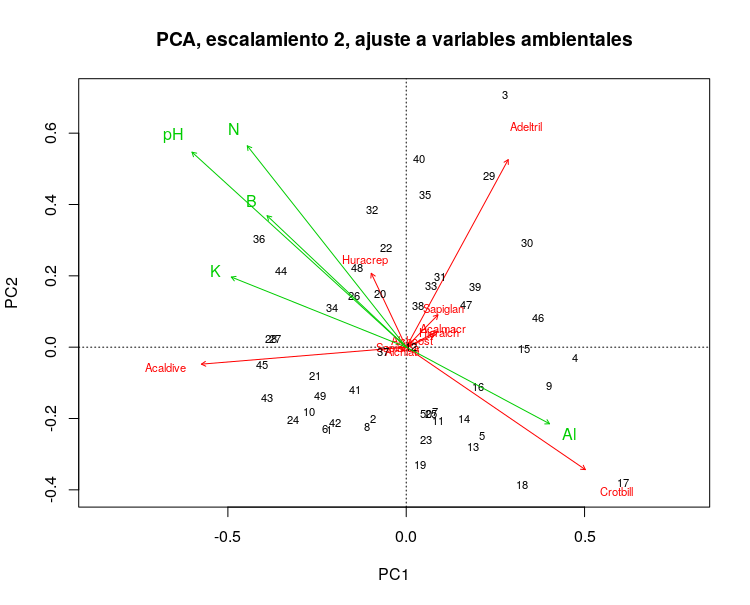
\includegraphics{suelo_especie.png}
\caption{\label{fig:suelo_especie}leyenda aqui}
\end{figure}

Si usamos solo las variables numéricas, obtendremos lo siguiente: N, Ph,
K, Al y B, siguen siendo variables significativas que pueden explicar la
distribución de especies,a las cuales se les suma Zn y Cu. También las
coordenadas UTM de este a oeste (UTM.EW) junto la riqueza global se
consideran variables significativas. En cuanto a la riqueza global, se
refiere al número de especie total por cuadro,la cual está asociado a la
matriz de comunidad como ya mencionamos, lo que significa que cuando
aumenta el número de especies, este puede ayudar a interpretar cómo se
distribuyen las especies dentro de la matriz de comunidad, dato que se
manifesto al principio en la correlacion de Pearson.(Ver
figura\ref{fig:geo_pearson}Correlacion de Pearson)

(ver figura\ref{fig:variables_numericas})

\begin{figure}
\centering
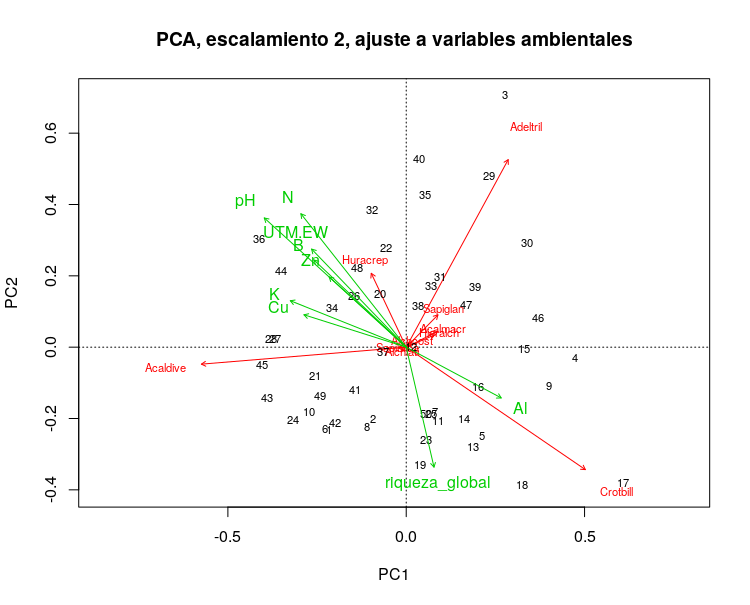
\includegraphics{variables_numericas.png}
\caption{\label{fig:variables_numericas}leyenda aqui}
\end{figure}

Una vez visto este análisis, pasemos al CA, análisis de correspondencia,
este es uno de los más usados y trata de llenar el vacío de las
limitaciones del PCA ya que este nos permite usar datos de conteos
aunque el CA no se puede aplicar a datos que no sean de frecuencias ya
sea de abundancia o de presencia ausencia y no es necesario transponer
las matrices. Está bien mencionar que en este análisis no trabajamos con
distancia Euclídea sino con la distancia ji-cuadrado.

Las distancias no van a coincidir del todo ya que se usan parámetros
diferentes pero de todas formas puede que resalten patrones ya vistos en
casos anteriores. El escalamiento 1 muestra la distancia en función de
sitios y el 2 la relación o distancia en función de especies.

Comencemos con el modelo de vara quebrada de nuestro CA, en este caso
los componentes CA2 y CA3, son los que podrían representar la matriz de
comunidad a diferencia de los demás modelos de vara quebrada donde el
componente 1 era el más explícito a nuestra matriz de comunidad.De todas
formas podemos usar las 4 primeras componentes para entender nuestra
matriz de comunidad y de esa forma entender y resumir el conjunto de las
multidimensiones de nuestra matriz de comunidad. Esto lo veremos mejor
explicado en los siguientes gráficos.

(ver figura\ref{fig:AC})

\begin{figure}
\centering
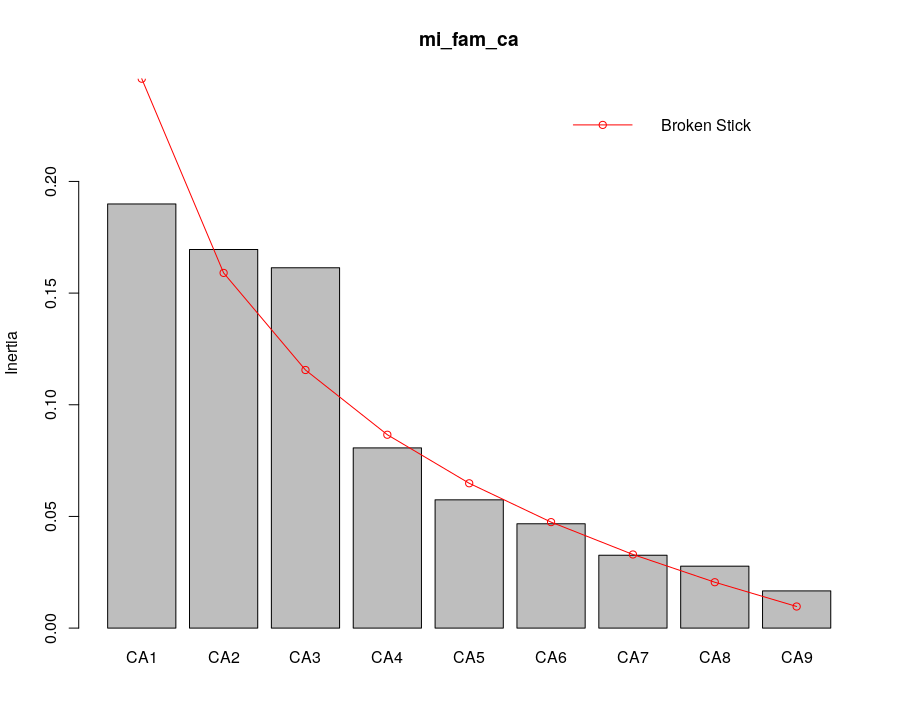
\includegraphics{AC.png}
\caption{\label{fig:AC}}
\end{figure}

Nuestros biplot del análisis de Correspondencia nos dicen lo siguiente:
no tenemos vectores, en este caso solo hay espacios comunes que muestran
la distribución y asociación. El biplot 1 o CA1 nos servirá para
entender la similitud entre sitios y viendo el gráfico nos dice que un
alto porcentaje de los sitios están más que relacionados,esto suele
pasar cuando nuestras especies no suelen ser tan especialistas, no
presentan patrones o tendencia muy clara. Hay unas 4 especies que rompen
este patrón: \emph{Adelia triloba}, \emph{Alchornea latifolia},
\emph{Acalypha macrostachya} y \emph{Sapium broadleaf}, en especial las
dos últimas, dándonos a entender que son especies algo más especialistas
y de poca abundancia, esto podemos evidenciarlo en la tabla de de
abundancia de especie por cuadrícula. (ver figura\ref{fig:abun_sp_q})

El biplot 2 nos servirá para ver la distancia entre especies, obtuvimos
lo siguiente: coincidiendo con el número 1, las especies guardan una
cercanía considerable, dando a entender que su patrón de distribución
podría ser homogéneo, aunque al igual que en el 1er biplot las especies
\emph{Adelia triloba}, \emph{Alchornea latifolia}, \emph{Acalypha
macrostachya} y \emph{Sapium broadleaf}, guardan una mayor distancia con
relación al resto, en especial las dos últimas, evidenciandola
consistencia entre los análisis.Las demás especies, por motivo de la
estrecha distancia ji-cuadrado, nos indica que están correlacionadas
entre sí.

En ambos biplots, \emph{Croton billbergianus} guarda cierta distancia
con relación a sitios y a especies, más en el 1er biplot que en el 2do,
pero no tanto como las especies antes mencionadas.

(ver figura\ref{fig:biplot_ca})

\begin{figure}
\centering
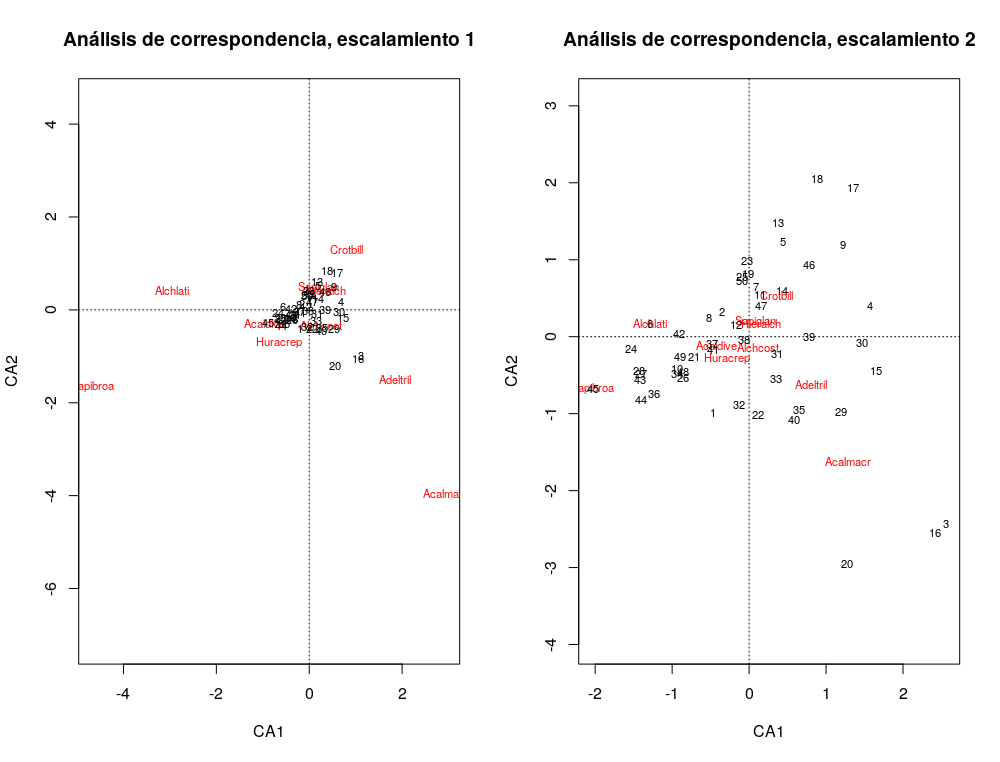
\includegraphics{biplot_ca.png}
\caption{\label{fig:biplot_ca}}
\end{figure}

Siguiendo con el PCoA o análisis de componentes principales en espa;ol,
este no usa la distancia euclídea ni la ji-cuadrada, lo que puede
resultar algo incómodo ya que esto nos resultara en vectores de
magnitudes negativas, imaginarias, dígase un vector complejo.Dicho
vector no se podrá aprovechar o representar como tal en el análisis de
coordenadas principales porque no se podrá representar en los ejes del
análisis.

Viendo los resultados de nuestro PCoA en el cual incluimos variables
ambientales y geomorfológicas, obtenemos lo siguiente: las especies que
muestran una contribución directa a sitios son, \emph{Sapium broadleaf}
que contribuye a los sitios 36,24,43 y 45, \emph{Alchornea latifolia} en
el sitio 48 y \emph{Adelia triloba} al sitio 19, aunque en la gráfica
las demás especies contribuyen no se muestran directamente asociadas a
un sitio en específico, estas contribuyen todos los sitios de manera
conjunta, también, las variables topográficas no muestras trascendencia
en este análisis a excepción de la heterogeneidad ambiental, riqueza
global y las coordenadas UTM de este a oeste (UTM.EW) que también se
hacen presente en los análisis anteriores.

Al igual que en los demás análisis, el Ph y el Nitrógeno (N) guardan
cierta relación pero en este caso se muestran una relación aún más
estrecha.

(ver figura\ref{fig:PCoA})

\begin{figure}
\centering
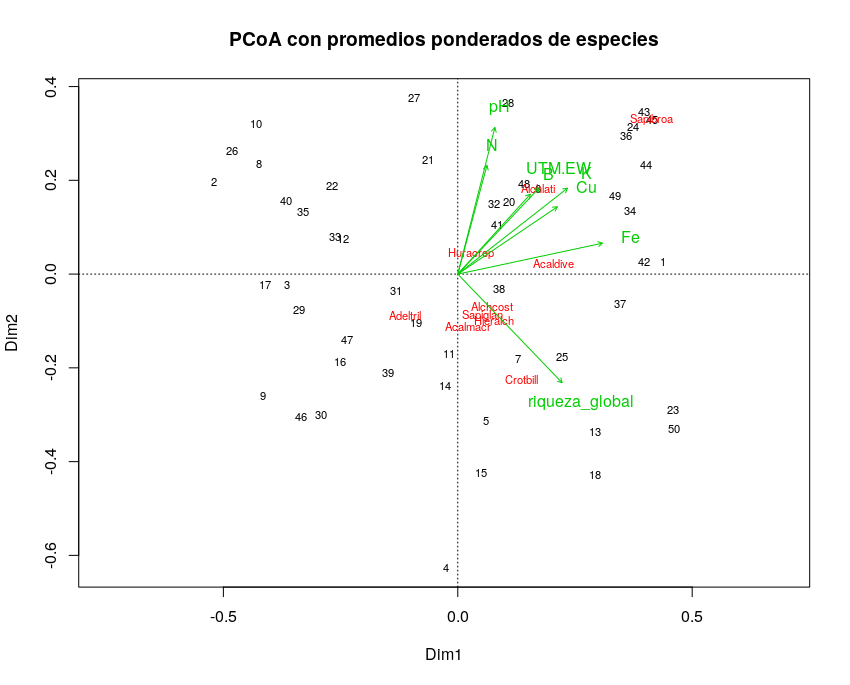
\includegraphics{PCoA.png}
\caption{\label{fig:PCoA}}
\end{figure}

TÉCNICA DE ORDENACIÓN RESTRINGIDA O CANÓNICA

En estas también integraremos variables ambientales o de suelo, especies
y sitios, como variables explicativas, para determinar su integración,
pero estas no tendrán la misma libertad de moverse a como lo hacían en
la Teco no restringida ya que estos análisis posee restricciones por
ajuste por medio de regresión lineal con respecto a la matriz ambiental,
en otras palabras, buscaremos tendencias en una matriz de comunidad
restringida péndolas a una matriz ambiental. Esto lo haremos a través de
2 de los principales análisis de la técnica de ordenación no
restringida, estos serán: análisis de redundancia o RDA (siglas de
\emph{Redundancy Analysis}) Y análisis de correspondencia canónica o CCA
(\emph{canonical correspondence analysis}).

Comencemos por RDA que es el hermano canónico el PCA, este es una
combinación de una regresión lineal múltiple y el análisis de
componentes principales dando como resultado múltiples variables de
respuesta (multivariado). En este la exploración de datos es explícita
relacionada a dos matrices, una de respuesta y una explicativa, en donde
la matriz de respuesta equivale a la matriz de comunidad y la matriz
explicativa equivale a la variable ambiental.

Los resultados del RDA son los siguientes: En el escalamiento uno lo que
hace sentido es la distancia euclídea, por lo cual, lo resultante es un
cúmulo de los sitios de forma cercana. y en el escalamiento 2 los
ángulos entre especies y variables. El escalamiento 1 se vería de la
siguiente manera: A pesar de que los números están apiñados, podemos
diferenciar ciertos clusters, por ejemplo: los sitios 1,2,5,7,8,15
formas un pequeño cluster que muestra una asociación con el Al
(aluminio), al igual que el 13,14,19, otro pequeño cluster asociado al
Al y 46 y 47 muestran estrecha relación con P (fósforo), también las
especies como \emph{Hura crepitans}, \emph{Acalypha
diversifolia},\emph{Croton billbergianus}, entre otras, están muy bien
explicadas en este escalamiento y bien representadas en los sitios
contiguos al vector.

(ver figura\ref{fig:RDA1_euclidea})

\begin{figure}
\centering
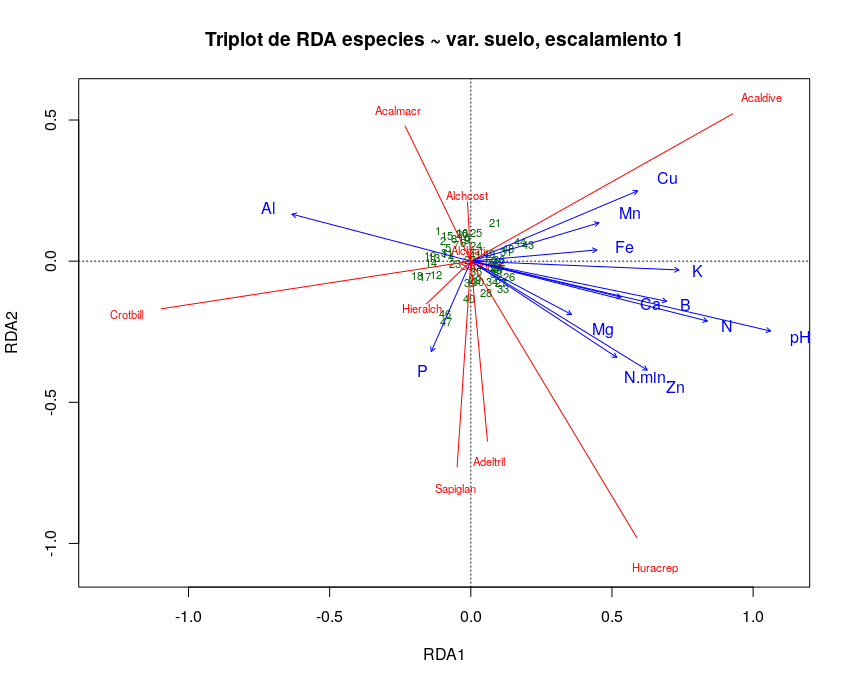
\includegraphics{RDA1_euclidea.png}
\caption{\label{fig:RDA1_euclidea}}
\end{figure}

Explicando la relación entre las variables explicativas en el
escalamiento 2, obtendremos lo siguiente: Las variables Ca,B,N y Ph,
muestran una estrecha relación entre sí, están presentes en los sitios
32,27 y 45 y que muestran una relación inversa con el aluminio
(Al).Tenemos un segundo cluster de Mg, Zn y N.min.(nitrógeno
mineralizado) con el Mg presente en el sitio 38, el Fe y K también
muestran cierta relación entre sí, en especial en los sitios 36,42,50,
el Mn y el Cu también están relacionados entre sí y presentes en los
sitios 31,43,44,48 y 49.

(ver figura\ref{fig:RDA})

\begin{figure}
\centering
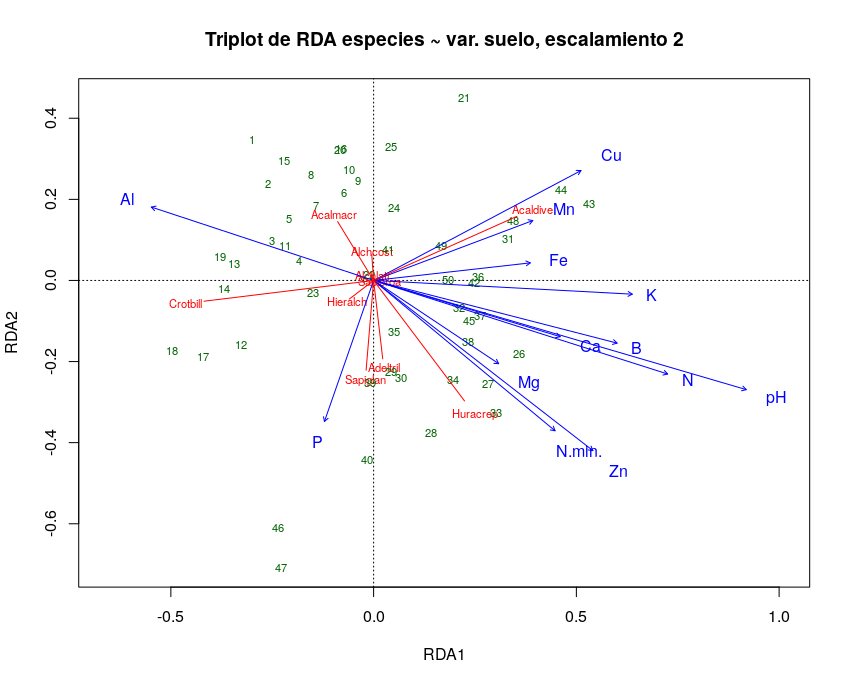
\includegraphics{RDA.png}
\caption{\label{fig:RDA}}
\end{figure}

También podemos añadir las variables que presentaron asociación en el
análisis pasivo de ordenación no restringida por PCA, y lo que vemos es
que aunque no existe colinealidad de forma directa, algunas variables
descriptivas forman ángulos bastante estrechos entre sí, indicando que
son variables muy relacionadas. Excluyendo variables asociadas al
analisis PCA de ordenacion no restringida, basandonos en los valores VIF
que estas poseen, el resultado es que: de cierta forma, el Al y el N.min
poseen una relacion inversa, las variables descriptivas B, N y Ph estan
relacionadas entre si de forma mas directa en los sitios 36, 39 y 44,
mientras que el Cu no muestra asociacion directa a las demas variables
explicativas pero si muestra constribucion a sitios como el
24,25,34,38,41,42 y 43.

(ver figura\ref{fig:PCA_RDA})

\begin{figure}
\centering
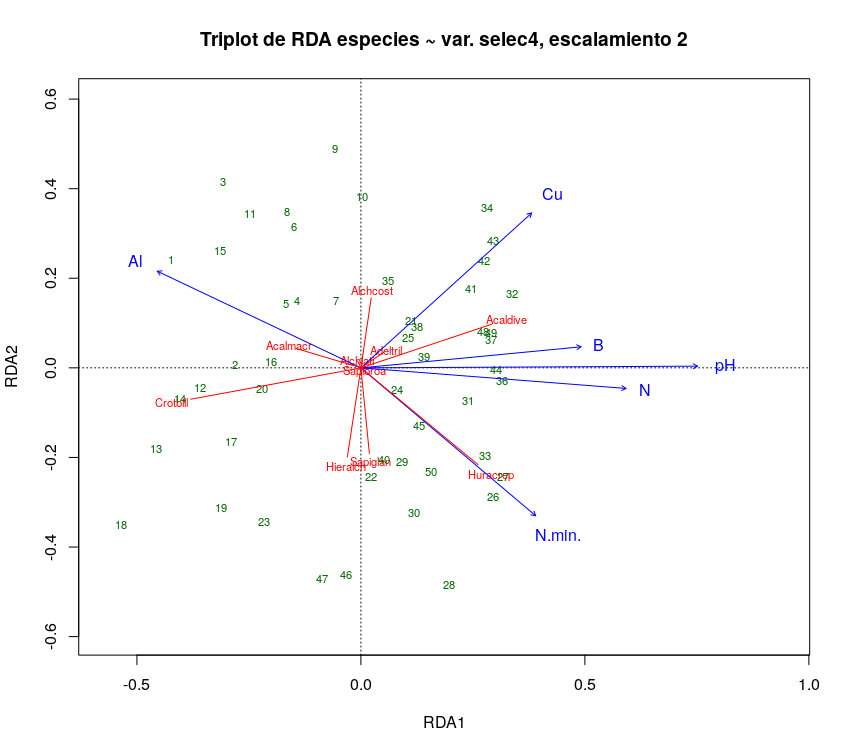
\includegraphics{PCA_RDA.png}
\caption{\label{fig:PCA_RDA}}
\end{figure}

Desde la perspectiva del nuestro segundo análisis de ordenación
restringida CCA, que es el hermano canonico del analisis de
correspondencia.en este analisis se relazo un ajuste a las variables
explicativas usando la distancia ji-cuadrado, de este tenemos los
siguientes resultados: en este caso la relacion inversa del Al es con el
N y el Ph, elementos que guardas una estrecha relacion entre si,
formando un cluster junto al B. El N.min aporta de forma directa a las
especies \emph{Hura crepitans} y \emph{Sapium broadleaf} per no muestra
estrecha relacion con otras variables explicativas, lo mismo pasa con el
Cu pero este aprota de forma mas directa a \emph{Adelia triloba}, esta
misma especie junto a \emph{Acalypha diversifolia} simulan ser especies
mienralizadas.

(ver figura\ref{fig:CCA})

\begin{figure}
\centering
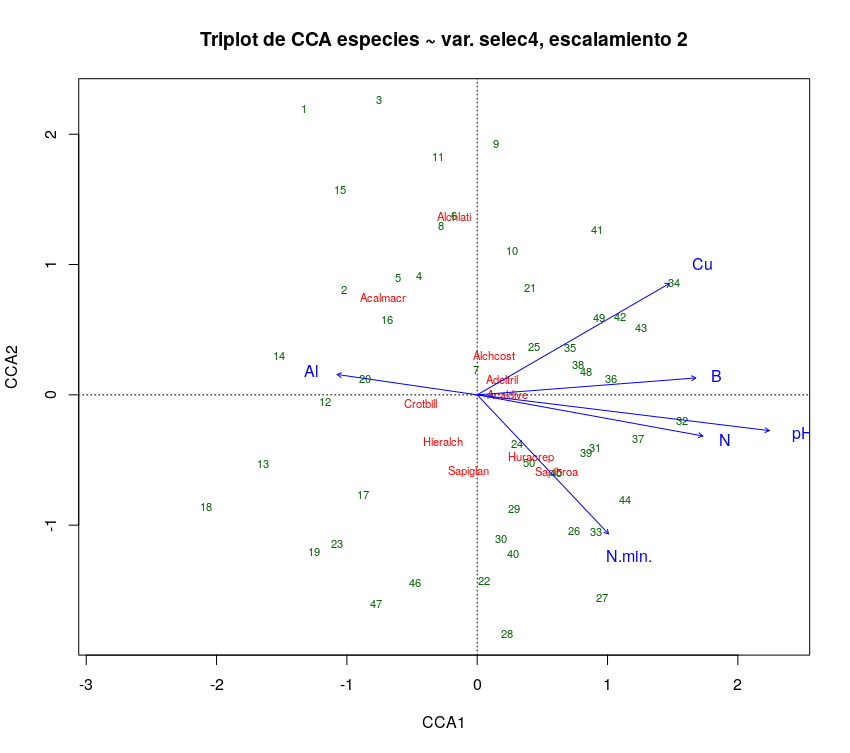
\includegraphics{CCA.png}
\caption{\label{fig:CCA}}
\end{figure}

Si mostraramos el mismo grafico pero sin especies ``raras'', tomano en
cuenta que el concepto raro en este caso esta aplicado a especies con
menos de 100 individuos, asi se explicaria mejor o estaria menos cesgado
los resultados con la distancia ji-cuadrado, tendiamos que nuestra
presicion pasaria de 0.1273683 a 0.1739327 y los resulados muestran que
en este caso la relacion inversa del Al se muestra con el Cu y el
N.min.,\emph{Acalypha diversifolia} sigue estando asociada al Ph y de
cierta forma aun guarda algun tipo de relacion con el N y el B.

(ver figura\ref{fig:no_raras})

\begin{figure}
\centering
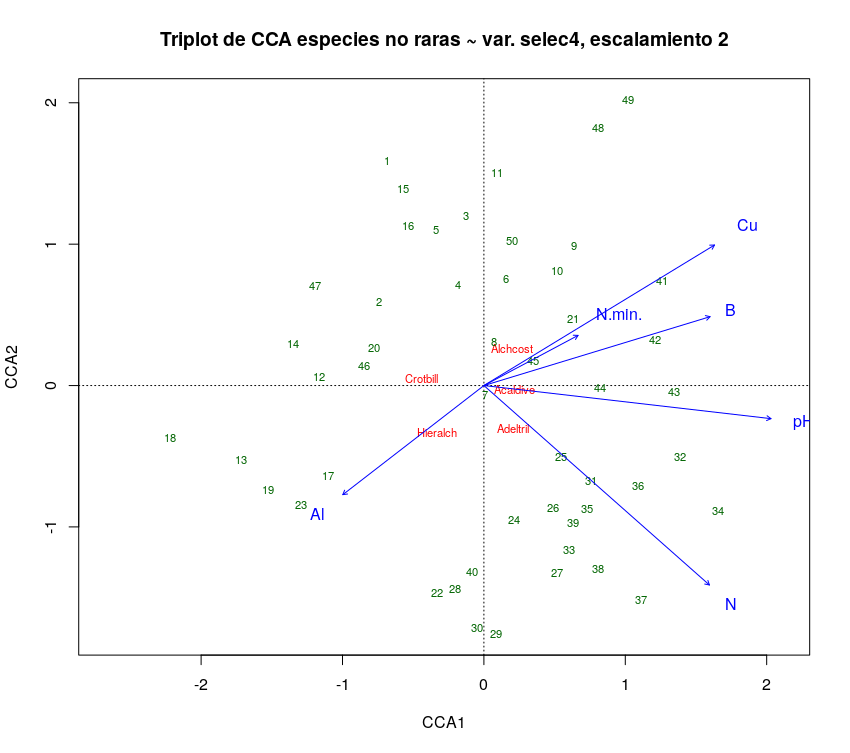
\includegraphics{no_raras.png}
\caption{\label{fig:no_raras}}
\end{figure}

OJO PAMELA!!! ( En resultados recuerda resaltar si la abundancia de
especies de euphorbeacia resulta comun,(``normla'')en panamá a pesar de
ser intertropical, cuando su mayor distribucion es tropical)

RECORDATORIO: EL AJUSTE POST-HOC DEL ANÁLISIS DE ORDENACIÓN SUGIERE QUE
LA VARIABLE pH (Y OTRAS) EXPLICA SIGNIFICATIVAMENTE LA COMPOSICIÓN DE
ESPECIES DE EUPHORBIACEAE. AMPLIAR HACIA VARIABLES GEOMORFOLÓGICAS,
UTILIZAR EL ANÁLISIS VIF PARA SELECCIONAR LAS VARIABLES EXPLICATIVAS Y,
NO OLVIDES, QUE LA ORDENACIÓN RESTRINGIDA DEBERÍA SER CONSISTENTE CON
ESTE ANÁLISIS. RECORDAR EXPLICAR LA ASOCIACIÓN ENTRE SITIOS MEDIANTE EL
GRÁFICO DE ESCALAMIENTO 1, LA RELACIÓN ENTRE VECTORES MEDIANTER ANGULO
EN EL GRÁFICO DE ESCALAMIENTO 2.

\ldots

\section{Discusión}\label{discusiuxf3n}

\section{Agradecimientos}\label{agradecimientos}

\section{Información de soporte}\label{informaciuxf3n-de-soporte}

\ldots

\section{\texorpdfstring{\emph{Script}
reproducible}{Script reproducible}}\label{script-reproducible}

\ldots

\section*{Referencias}\label{referencias}
\addcontentsline{toc}{section}{Referencias}

\hypertarget{refs}{}
\hypertarget{ref-condit1998tropical}{}
Condit, R. (1998). \emph{Tropical forest census plots: Methods and
results from barro colorado island, panama and a comparison with other
plots}. Springer Science \& Business Media.

\hypertarget{ref-condit1999dynamics}{}
Condit, R., Ashton, P. S., Manokaran, N., LaFrankie, J. V., Hubbell, S.
P., \& Foster, R. B. (1999). Dynamics of the forest communities at pasoh
and barro colorado: Comparing two 50--ha plots. \emph{Philosophical
Transactions of the Royal Society of London. Series B: Biological
Sciences}, \emph{354}(1391), 1739--1748.

\hypertarget{ref-condit1995mortality}{}
Condit, R., Hubbell, S. P., \& Foster, R. B. (1995). Mortality rates of
205 neotropical tree and shrub species and the impact of a severe
drought. \emph{Ecological Monographs}, \emph{65}(4), 419--439.

\hypertarget{ref-hubbell1999light}{}
Hubbell, S. P., Foster, R. B., O'Brien, S. T., Harms, K. E., Condit, R.,
Wechsler, B., \ldots{} De Lao, S. L. (1999). Light-gap disturbances,
recruitment limitation, and tree diversity in a neotropical forest.
\emph{Science}, \emph{283}(5401), 554--557.

\hypertarget{ref-meyer2013detecting}{}
Meyer, V., Saatchi, S., Chave, J., Dalling, J., Bohlman, S., Fricker,
G., \ldots{} Hubbell, S. (2013). Detecting tropical forest biomass
dynamics from repeated airborne lidar measurements.
\emph{Biogeosciences}, \emph{10}(8), 5421.




\newpage
\singlespacing 
\end{document}
